% TODO JAMES O runtime online is different to empirical findings

% TODO mention point cloud somewhere

% TODO END go through lindard and l90 reports
% TODO END percentage of data values, consistent term
% TODO END present/past
% TODO END check for emotional language
% TODO END as -> since
% TODO comment code
% TODO random forest(s) sp.
% TODO END citations: make sure author is mentioned, If you use purely-numeric bibliographic references, do not forget to still mention authors’ surnames

% TODO ----------------------------------------------------------------

\documentclass[a4paper,12pt,twoside,openright]{report}

\usepackage{graphicx}

\def\authorname{Jan S\"ondermann\xspace}
\def\authorcollege{Selwyn College\xspace}
\def\authoremail{jjes2@cam.ac.uk}
\def\dissertationtitle{Bayesian optimisation of approximateness in the trade-off between statistical and computational efficiency}
% TODO END word count
\def\wordcount{@}

\usepackage{todonotes}
\usepackage{euscript}
\usepackage[export]{adjustbox}
\usepackage{subcaption}
\usepackage{chngpage}
\usepackage{calc}
\usepackage{epsfig,graphicx,parskip,setspace,tabularx,xspace} 
\usepackage{enumitem}
\usepackage{mathtools}
\usepackage{amsmath,amssymb}
\usepackage{algorithmicx}
\usepackage{algorithm}
\usepackage{algpseudocode}
\newcommand{\Break}{\State \textbf{break} }
\usepackage{listings}
\lstset{breaklines=true, frame=single, numbers=left, basicstyle=\small\ttfamily}

\DeclareMathOperator*{\argmax}{arg\,max}


%% START OF DOCUMENT
\begin{document}


%% FRONTMATTER (TITLE PAGE, DECLARATION, ABSTRACT, ETC) 
\pagestyle{empty}
\singlespacing
% title page information
\begin{titlepage} 

\begin{center}
\noindent
\huge
\dissertationtitle \\
\vspace*{\stretch{1}}
\end{center}

\begin{center}
\noindent
\huge
\authorname \\
\Large
\authorcollege      \\[24pt]

\includegraphics{CUni3.eps}
\end{center}

\vspace{24pt} 

\begin{center}
\noindent
\large
{\it A dissertation submitted to the University of Cambridge \\ 
in partial fulfilment of the requirements for the degree of \\ 
Master of Philosophy in Advanced Computer Science} 
\vspace*{\stretch{1}}
\end{center}

\begin{center}
\noindent
University of Cambridge \\
Computer Laboratory     \\
William Gates Building  \\
15 JJ Thomson Avenue    \\
Cambridge CB3 0FD       \\
{\sc United Kingdom}    \\
\end{center}

\begin{center}
\noindent
Email: \authoremail \\
\end{center}

\begin{center}
\noindent
\today
\end{center}

\end{titlepage} 

\newpage
\vspace*{\fill}

\onehalfspacing
\newpage
{\Huge \bf Declaration}

\vspace{24pt} 

I \authorname of \authorcollege, being a candidate for the M.Phil in
Advanced Computer Science, hereby declare that this report and the
work described in it are my own work, unaided except as may be
specified below, and that the report does not contain material that
has already been used to any substantial extent for a comparable
purpose.

\vspace{24pt}
Total word count: \wordcount

\vspace{60pt}
\textbf{Signed}: 

\vspace{12pt}
\textbf{Date}:


\vfill

This dissertation is copyright \copyright 2010 \authorname. 
\\
All trademarks used in this dissertation are hereby acknowledged.



\newpage
\vspace*{\fill}

\singlespacing
\newpage
{\Huge \bf Abstract}
\vspace{24pt} 


% TODO write abstract
%Our project falls into the field of meta-machine learning that tries to use machine learning methods to improve the result of using these methods.


\newpage
\vspace*{\fill}




\pagenumbering{roman}
\setcounter{page}{0}
\pagestyle{plain}
\tableofcontents
\listoffigures
\listoftables
\listoftodos

\onehalfspacing


\chapter{Introduction}

\pagenumbering{arabic}
\setcounter{page}{1}

Before the advent of computers, statistical methods had to be simple enough to be calculable by hand which greatly limited the degree of complexity that these methods could reach. As computing power available to statisticians increased, many new methods were devised to make use of these new resources, in some cases exceeding the computational possibilities available.

Although machine learning is a very diverse subject that combines influences from many different fields such as engineering, computer science, computational biology and physics, many of the recent advances have come from statistics or made use of statistical methods. As is true for mathematics more generally, considerations of runtime and complexity are usually not in the focus of attention of statistical research. This is a stark contrast to computer science where the analysis of algorithmic complexity has been of great importance since the early beginnings of the field.

The cultural differences between computer science and statistics is revealed in the attitudes towards data that these fields exhibit: while in computer science, data is seen as a workload to be completed, in statistics, the perception is that more data is something desirable, allowing higher confidence in inferential results.

In recent years, the amount of scientific and commercial data available has increased rapidly, a phenomenon often labeled "Big Data". As data science experts are facing the task of analysing these large datasets, controlling runtime has become increasingly important.

The current states of the field of machine learning requires skilled humans to make high level decisions on trade-offs between computational and statistical efficiency such as when to use approximate inference methods or when to use a simple method with lots of data rather than a complex method with a small amount of data. 

The necessary knowledge to make adequate decisions in these cases is often acquired through experience and an intuitive familiarity with the learning algorithms that can be hard to formalise and teach. As part of the current trend to automise all aspects of machine learning, automating the process of finding an optimal balance in these trade-offs would be an important contribution to the field.


One way to add runtime considerations to statistical learning is to construct anytime algorithms \cite{conf/aaai/DeanB88}. Algorithms of this kind produce successively better results during the course of their execution. They can be terminated early, returning a result whose quality depends on the time they were allowed to run for.

Another useful type of algorithms that require an understanding of runtime are contract algorithms \cite{ZCCijcai99} that expect a dataset and a time budget as input and infer an optimal model within the time budget.



Given an algorithm with a number of "approximation parameters" that control the degree of approximateness at which the algorithm runs, these algorithms can be understood as optimisation problems. They find optima of the function taking the approximation parameters to the time and predictive accuracy of the learning algorithms. In the process of optimisation, they have to take account of the additional runtime constraints that exist.

Classical optimisation methods may be ineffective in these cases as evaluating the function to be optimised can be very expensive to compute. Further complicating this problem is the fact that the time required to evaluate the function can vary drastically depending on where it is evaluated: consider the case where the approximation parameter is the number of layers in a deep neural network. Increasing the number of layers will cause the inference to take more time. The optimisation routine has to take this into account when exploring the function. 

A natural solution to this problem is Bayesian optimisation as Bayesian optimisation methods make very efficient use of data when optimising a function.


Our first major contribution in this project is a model of how approximation parameters affect learning algorithm time and score. This model forms the foundation for the second major contribution of our system, a number of heuristics that use Bayesian optimisation methods to solve anytime and contract style problems as described above.



\begin{figure}
\centering
  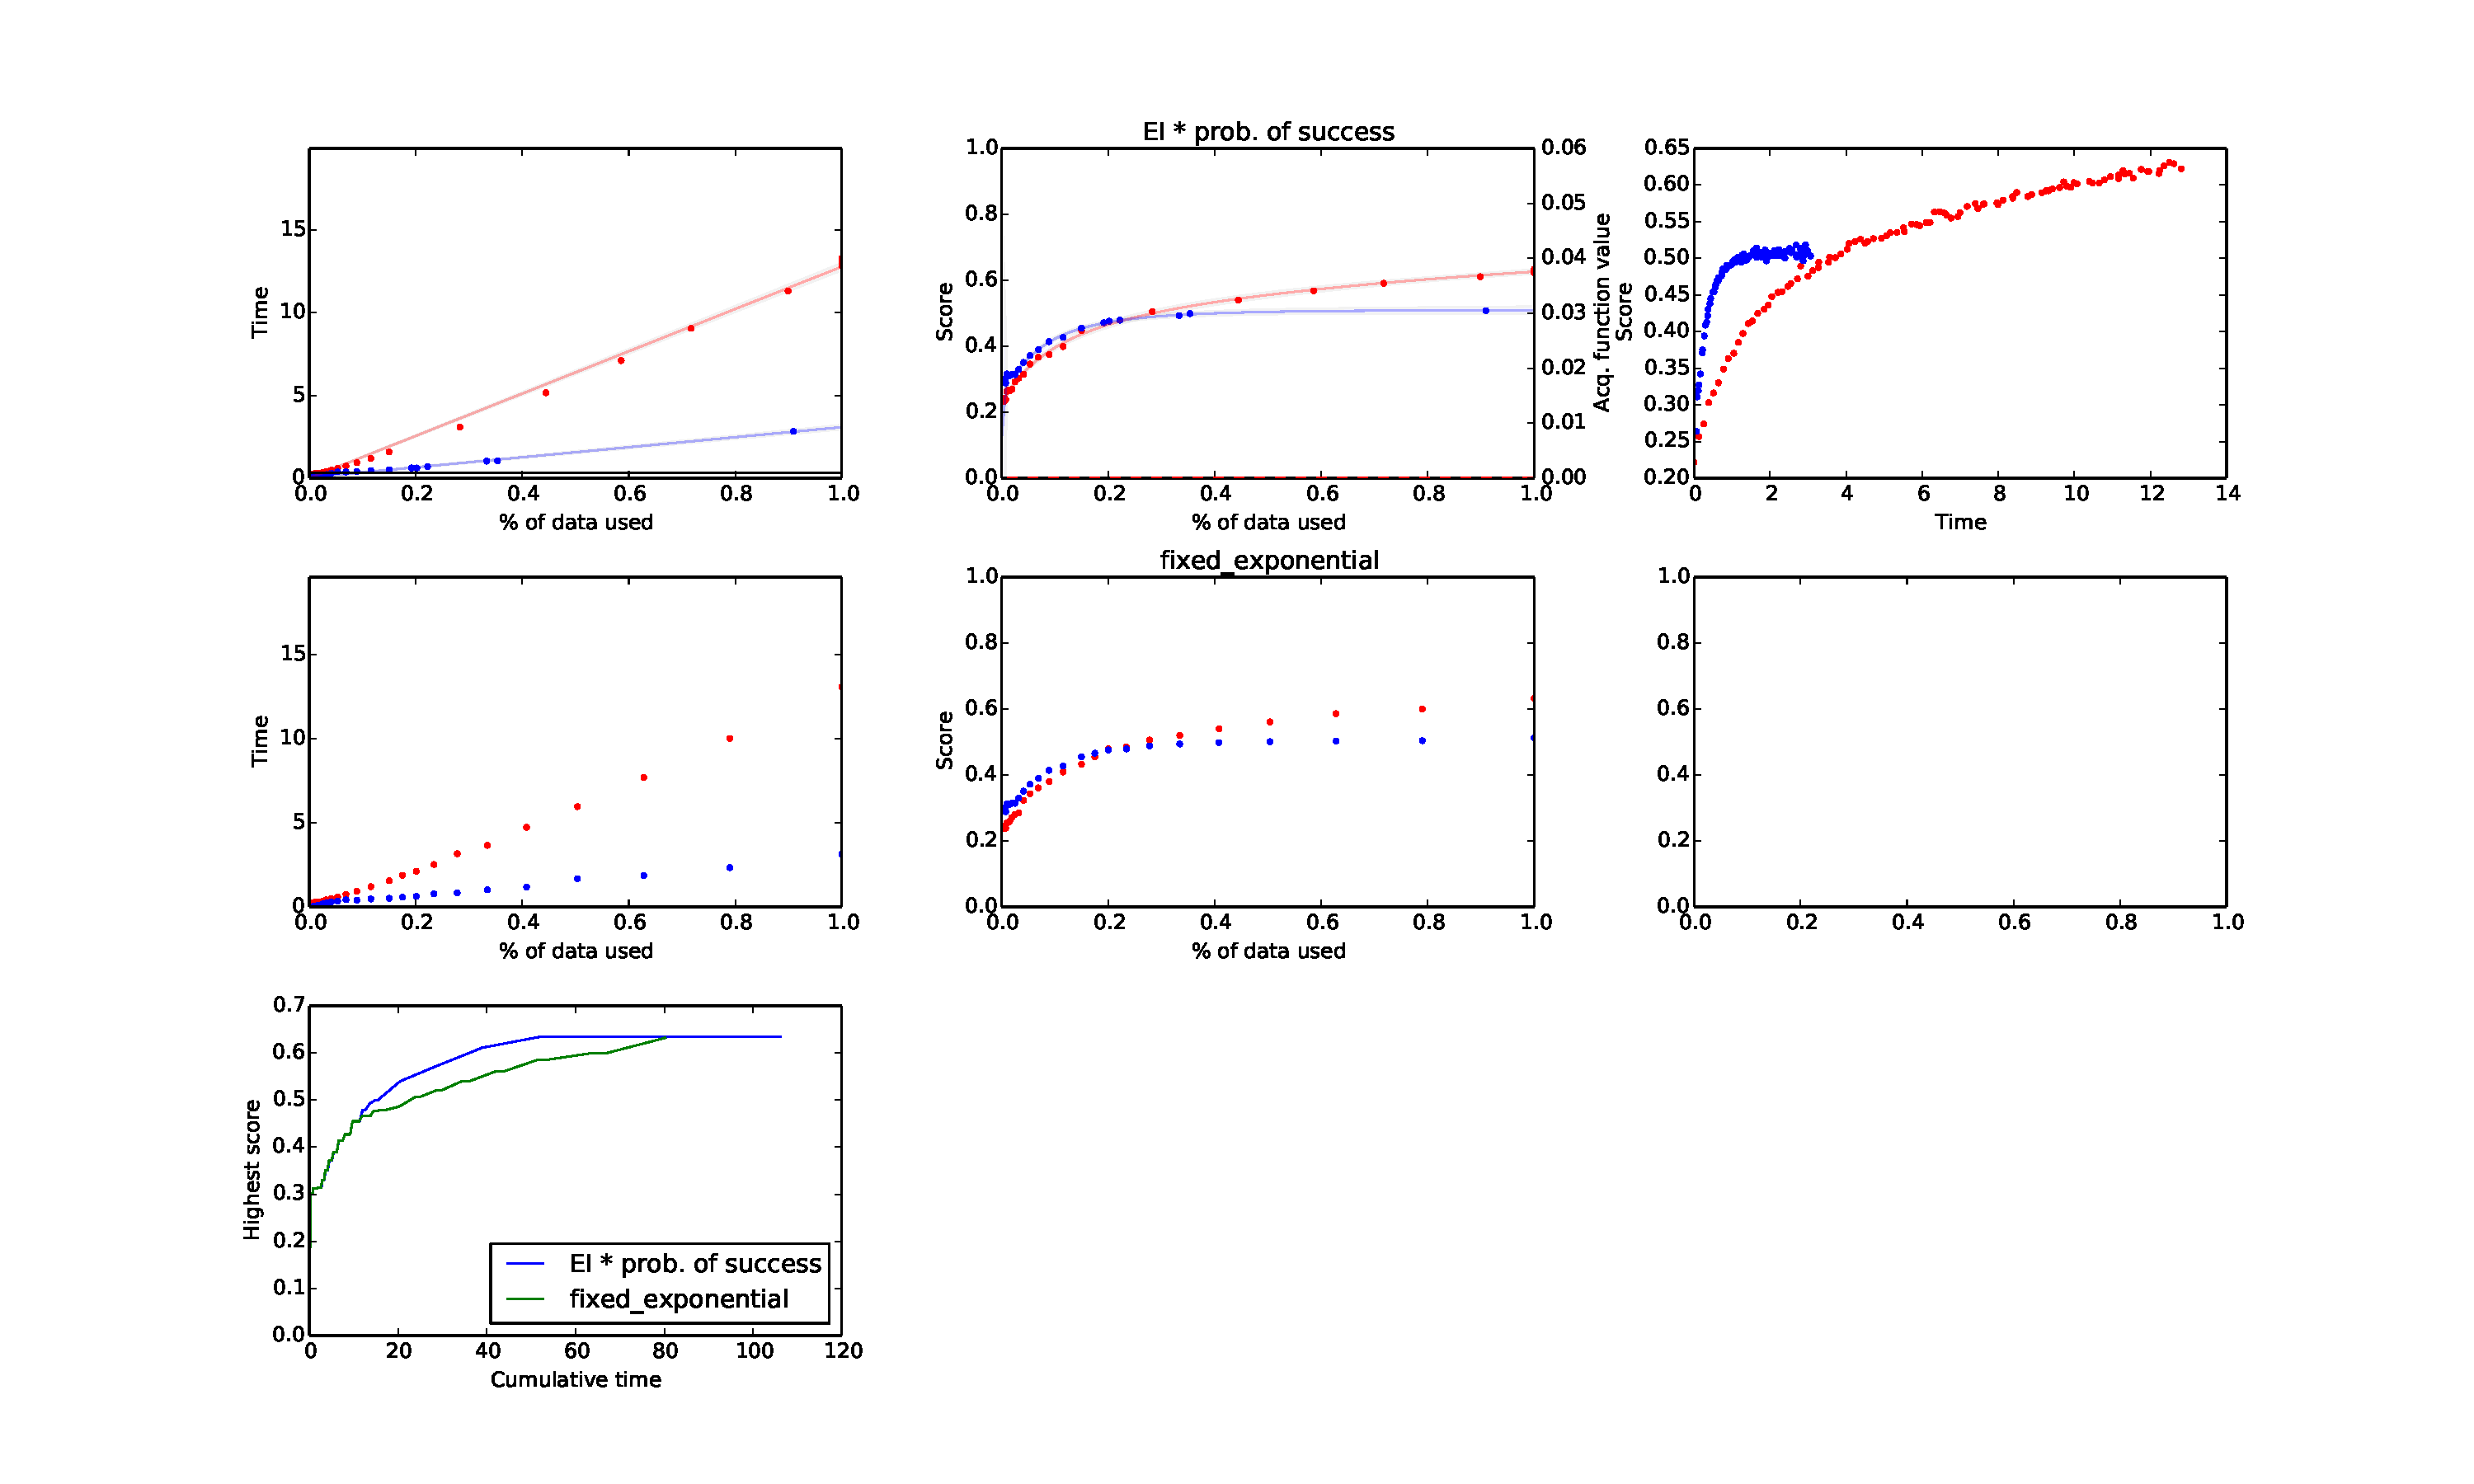
\includegraphics[trim=130 40 910 560,clip,width=\textwidth]{figures/anytime1.pdf}
  \caption{Comparing two heuristics}
  \label{anytime1}
\end{figure}


Figure \ref{anytime1} shows a plot that compares the performance of two anytime heuristics running in parallel. The $x$-axis shows the time in seconds that has elapsed since the start of the program while the $y$-axis shows the classification accuracy of the best model the heuristics have found. The "\texttt{fixed\_exponential}" heuristic (shown in green) is a naive implementation that simply tries a fixed sequence of values for the approximation parameter. The "\texttt{EI * prob.\ of success}" heuristic (shown in blue) is a more advanced heuristic which is explained in detail below. 

Both heuristics spend about 10 seconds in a burn-in phase in which they build the same models. After this burn-in ends, the blue heuristic immediately starts producing better models green heuristic and plateaus out at the maximum value about 50 seconds after learning starts. To reach the same classification accuracy, the naive heuristic needs about 80 seconds.

Although both heuristics reach the same final accuracy eventually, if we terminate them after 30 seconds, the best model found by the "\texttt{EI * prob of success}" is substantially better than that found by the naive heuristic at this point which makes it a better anytime algorithm. 

Besides this anytime heuristic, we also describe a contract heuristic that constructs models in a time budget it is given.


The remainder of this report is structured as follows:
\begin{itemize}
	\item The \textbf{Background} chapter introduces the theoretical ideas that this project is built on. It also lists the third-party technologies that were used during development
	\item The \textbf{Related Work} summarises the current state of research regarding the problems we are trying to solve
	\item The \textbf{Modelling Learning Time and Score} chapter explains how we model the performance of the learning algorithms using Gaussian processes
	\item The \textbf{Scheduling} chapter describes the architecture of the software we have written. It also lists and explains the heuristics we developed
	\item The \textbf{Evaluation} section examines what we have built by describing and evaluating results. It also lists challenges we faced and limitations of our current implementation
	\item The \textbf{Conclusion and future work} recapitulates our results by returning to the broader context lined out in this introduction and lists possible ways of extending the existing system
\end{itemize}






\chapter{Background}
\textit{This chapter describes the background assumed in the remainder of the document. We give a brief explanation of general machine learning principles together with a summary of the algorithms used in this project, including Gaussian processes which form the basis of the Modelling chapter. We then describe Bayesian optimisation which is the method underlying the ideas described in the Schedulers chapter, and briefly mention third-party software we used to build our system.}


\section{Key Concepts}
\begin{figure}
\centering
  \includegraphics[width=\textwidth]{figures/ml.pdf}
  \caption{The general process of learning from data}
  \label{mlstructure}
\end{figure}

Our project falls into the field of meta machine learning. We use machine learning algorithms to learn and predict the performance of other machine learning algorithms. This necessitates a very brief overview of machine learning principles: Figure \ref{mlstructure} shows the general structure of learning from data: a learning algorithm takes some training data and outputs a function $\hat{f}$, usually called a model of the data, that models the true function $f$ underlying the data. This function is then used to make predictions on unseen data.

Of particular relevance to our project is the second input to the learning algorithm: its hyperparameters. These hyperparameters control the behaviour of the learning algorithm and influence the quality of the model which makes selecting appropriate hyperparameters crucial.


\subsection{Approximation Parameters}
By "approximation parameters", we denote parameters to machine learning algorithms that influence the trade-off between statistical and computational efficiency, letting us vary the degree of approximateness at which the algorithm runs. Changing an approximation parameters should either decrease the runtime at the cost of classification accuracy or improve accuracy while making training slower. 

The approximation parameter that we put most of our focus on in this project is the proportion of the available data. Other approximation parameters are hyperparameters to the machine learning algorithms such as the number of decision trees in a random forest. This parameter is considered in the Modelling chapter to analyse how multiple interaction parameters interact.

Note that not all hyperparameters are approximation parameters. Some hyperparameters influence performance without changing the runtime such as the length-scales of Gaussian process kernels, explained in depth in the Gaussian process section of this chapter.\footnote{Many machine learning packages include parameters such as the number of threads used for learning in their API. These are parameters that influence runtime but not performance. They are, however, particular to the implementation and not part of the algorithm.}

\subsection{Scheduling}
As mentioned in the introduction, the problem we try to solve in this project is an optimisation problem with the additional component of runtime constraints. A solution to this problem consists in devising strategies to decide on a sequence of evaluations of the function to be optimised such that we find an optimum within these constraints. 

We use the term "scheduler" to denote heuristics that are used to select such a sequence. Schedulers allocate the time available to the models bulit during optimisation.

\subsection{Time, Score and Performance}
The learning algorithm can be assessed in two ways: the time it takes to create a model and the quality of its prediction. We denote this predictive strength by "score" and call both the time and score together the algorithms "performance".

\section{Machine Learning Algorithms}
\subsection{Logistic Regression and Random Forest}
This subsection introduces the two machine learning algorithms that we focus on in the evaluation of our system, logistic regression and random forests. These two algorithms are among the most common machine learning algorithm and are frequently used in real world applications.

\subsubsection{Logistic regression}

Logistic regression is a variant of linear regression, a very widely used machine learning algorithms. In linear regression, the model $\hat{f}$ has the form
\begin{equation}
\hat{f}(\mathbf{x}) = \mathbf{w}_0 + \sum_{i=1}^n \mathbf{w}_i \mathbf{x}_i
\end{equation}

where the vector $\mathbf{w}$ contains the model parameters and $n$ is the number of features. Fitting the model to data is achieved by adapting these parameters.

Linear regression is used for regression problems, where the values to be predicted are continuous. The datasets we consider in this report belong to a different type, where the required output is a label taken from a finite set of classes.

In the simplest case of such classification problems, binary classification, where each sample belongs to one of two classes, we wrap the computation of $\hat{f}$ in a function that forces all values into the range from 0 to 1. A commonly used function with this property is the sigmoid function $\sigma(x) = \frac{1}{1+e^x}$. We then assign the classes to 0 and 1, such that values for $\hat{f}$ close to 1 are to be interpreted to mean that the sample is likely to be of class 1.

In the multiclass case with $c$ classes, the machine learning library used in this project, described in detail below, constructs $c$ functions $\hat{f}^{(c)}$. Each function performs a binary classification between the class with index $c$ and all other classes, such that for samples likely to belong to class with index $c$, $\hat{f}^{(c)}$ has values close to 1. $\hat{f}$ is then computed by selecting the class for which $\hat{f}^{(c)}$ is largest. This technique is known as one-vs-all.

\subsubsection{Random forests}
Random forests, introduced in \cite{rndforests}, is an algorithm that extends the idea of decision trees, a simple learning method. Decision trees are grown by repeatedly splitting the feature space into rectangular regions such that a the proportion of samples of the same class in the region is maximised \cite{james2014introduction}. 

Individual decision trees alone can not compete with the predictive performance of other algorithms. In particular they suffer from high variance which means that multiple trees created using the same dataset often make very different predictions. An initial solution to this, proposed in \cite{bagging}, is Bagging, a technique that creates a number of new training sets by drawing samples from the original dataset. The trees are then fitted to these new training sets. To make a prediction, the predictions of all trees are averaged over.

Random forests improve the results obtained by bagging through decorrelating the trees. This is achieved by only considering a subset of features from the full set of features at each training step. This prevents the trees from choosing the same features in the same order. By combining and averaging over a set of decision trees as described, random forests achieve a performance that makes them a popular choice in machine learning.

The number of trees is a possible approximation parameter to random forests. Another hyperparameter that is also an approximation parameter is the minimum number of samples that must be contained in each region of the feature space for the trees in the forest.

\subsection{Gaussian Processes}
Gaussian processes are a machine learning method commonly used for regression problems. Unlike methods such as logistic regression or random forests that learn by updating a set of model parameters, Gaussian processes place a prior directly over the function $\hat{f}$ \cite{Murphy:2012:MLP:2380985}. For this reason, they belong to the nonparametric family of learning algorithms. This prior is updated to a posterior based on the training data using Bayes' theorem.

If we think of functions as infinitely sized vector indexed by the domain of the function, Gaussian processes can be understood as a generalisation of the multivariate Gaussian distribution to a distribution over infinitely many variables. Formally, a multivariate Gaussian distribution $\mathcal{N}(\mu, \Sigma)$ is specified by a mean vector $\mu$ and a covariance matrix $\Sigma$. Equivalently, a Gaussian process $\EuScript{G}\EuScript{P}(m, \kappa)$ is specified by a mean function $m(x)$ and a covariance function $\kappa(x, x')$ (if we think of infinite vectors as single valued functions, infinitely large matrices can be seen as functions with two arguments). It is common for the mean function to be a constant function with $\mu(x) = 0$ as the mean can be included in the covariance function. Covariance functions are also commonly called kernels. We will use the two terms interchangeably.

If we draw a function $f \thicksim \EuScript{G}\EuScript{P}(m, \kappa)$ from a Gaussian process, every finite set of inputs to the function $\mathbf{x} = (x_1, \cdots, x_n)$ span a multivariate Gaussian distributed vector $\mathbf{f} = (f(x_1), \cdots, f(x_n)) \thicksim \mathcal{N}(\mu,K)$ with $\mu = (m(x_1), \cdots, m(x_n))$ and $K_{ij} = \kappa(x_i, x_j)$ \cite{Rasmussen:2005:GPM:1162254}.

To encode prior assumptions about the nature of the functions to be modelled by a Gaussian process, one chooses a covariance function that expresses these assumptions by assigning appropriate covariances. There is a set of commonly used covariance functions that Gaussian process libraries usually implement. In the remainder of this section, we explain how prior information is reflected in the kernels, following \cite{duvenaudthesis} in our explanations. We will return to this topic in the Modelling chapter when we describe the implementation of a custom covariance function. 

\subsubsection{The squared exponential kernel}
The squared exponential kernel is often chosen as a default kernel in Gaussian process modelling and, as such, very widely used. This kernel defines $\kappa(x, x') = \sigma_f^2 \text{exp}(-\frac{(x-x')^2}{2\ell^2})$ with $\sigma_f^2$ being the variance of the function and $\ell$ being the characteristic length-scale of the kernel. Figure \ref{sekernel} shows how the value of the squared exponential kernel changes as $x'$ moves away from $x$. 

The value of $\kappa(x, x')$ can be interpreted as the degree of similarity between $f(x)$ and $f(x')$ with larger values of $\kappa$ meaning higher similarity. This means that the squared exponential kernel expresses the prior that the functions to be modelled by the Gaussian process will be smooth. Precisely how smooth they will be is determined by the length-scale $\ell$. This is a hyperparameter to the squared exponential kernel. These hyperparameters allow separating general assumptions, such as "the functions will be smooth", from specific degrees of "smoothness". Figure \ref{sekernel_ls} shows how changing the value of $\ell$ influences the shape of the kernel function.

\begin{figure}
\centering
  \includegraphics[trim=120 240 100 230,clip,width=.4\textwidth]{figures/se_kernel.pdf}
  \caption{The squared exponential kernel with $x$ fixed in the center and $x'$ varying}
  \label{sekernel}
\end{figure}

\begin{figure}
\centering
  \includegraphics[trim=120 240 100 230,clip,width=.4\textwidth]{figures/se_kernel_different_ls.pdf}
  \caption{Three different values for $\ell$ in the squared exponential kernel with $x$ fixed in the center and $x'$ varying}
  \label{sekernel_ls}
\end{figure}

Figure \ref{sekernel_draws} shows five functions drawn from a Gaussian process with a squared exponential kernel and $\sigma_f^2 = \ell = 1$. Note how although the functions take different value, they share the same degree of smoothness. Figure \ref{sekernel_draws_different_ls} shows the effect that varying $\ell$ has on the functions: for smaller values, the functions become more rugged while increasing $\ell$ makes the function even smoother.


\begin{figure}
\centering
  \includegraphics[trim=120 240 100 230,clip,width=.6\textwidth]{figures/se_kernel_draws.pdf}
  \caption{Five draws from a Gaussian process with a squared exponential kernel}
  \label{sekernel_draws}
\end{figure}

\begin{figure}
\centering
  \includegraphics[trim=120 240 100 230,clip,width=.6\textwidth]{figures/se_kernel_draws_different_ls.pdf}
  \caption{Functions drawn from Gaussian processes with squared exponential kernels that have different length-scales}
  \label{sekernel_draws_different_ls}
\end{figure}

The squared exponential kernel is an example of a class of kernels called \emph{stationary kernels}. These kernels  have the property that their value does not change if $x$ and $x'$ are shifted by the same amount. Formally, for stationary kernels, $\kappa(x, x') = \kappa(\tau + x, \tau + x')$. This means that the smoothness of functions drawn from a Gaussian process with a squared exponential kernels does not change globally.


\subsubsection{The linear kernel}
The linear kernel is defined as $\kappa(x, x') = \sigma_f^2(x-c)(x'-c)$ with $c$ determining the $x$-coordinate of the point that all the functions in the posterior pass through \cite{duvenaudthesis}. The linear kernel is an example of a kernel that is not stationary as it models global, linear change in the functions.


\subsubsection{Combining kernels}
Although there is a substantial number of such common kernels, their number is still finite. To express more complex priors, it is therefore necessary to combine existing kernels to form new ones. One way to do so is to add them together. Figure \ref{sum_of_lin_and_se} shows functions drawn from a Gaussian process that has as its kernel the sum of a squared exponential and a linear kernel. It combines a linear component with the noisiness of the squared exponential kernel.

\begin{figure}
\centering
  \includegraphics[trim=80 210 70 195,clip,width=.6\textwidth]{figures/sum_of_lin_and_se.pdf}
  \caption{Adding a linear kernel to a squared exponential kernel}
  \label{sum_of_lin_and_se}
\end{figure}

Another way to combine kernels is multiplication. Figure \ref{prod_of_lin_and_lin} shows the result of multiplying to linear kernels together, which results in quadratic functions.

\begin{figure}
\centering
  \includegraphics[trim=80 210 70 195,clip,width=.6\textwidth]{figures/prod_of_lin_and_lin.pdf}
  \caption{Multiplying two linear kernels}
  \label{prod_of_lin_and_lin}
\end{figure}

\subsubsection{Marginal Likelihood}
The marginal likelihood of some data $y$ for a Gaussian process given data $\mathcal{D}$ and hyperparameters $\theta$ is obtained by integrating over the functions $f$ that the Gaussian process defines a distribution over. Formally:
\begin{equation}
p(\mathbf{y}|\mathcal{D}, \theta) = \int p(\mathbf{y}|f, \mathcal{D}, \theta)p(f|\mathcal{D}, \theta) df
\end{equation}

Comparing the marginal likelihood of two models allows us to choose the one that better fits the data.

\section{Bayesian Optimisation}
Bayesian optimisation is a method to solve the optimisation problem of having to find an $x$ that maximises\footnote{We will consider maximisation only in this section as minimising $f$ is equivalent to maximising $-f$} $f(x)$ for a given function $f$, commonly written 
\begin{equation}
\argmax_x f(x)
\end{equation}

Bayesian optimisation is based on the idea of placing a prior over the function $f$. After evaluating $f$ and obtaining a new data point, the model of $f$ is updated an used to decide where to evaluate the function next.

As Gaussian processes are precisely such priors over functions, they are very well suited to be used with Bayesian optimisation. By selecting an appropriate kernel as described in the previous section, one can express existing prior knowledge over the function to be optimised which is crucial in ensuring that the Bayesian optimiser makes good choices in deciding the sequence of function evaluations.

Unlike other optimisation methods like gradient descent that only use information local to the function at the last evaluation, Bayesian optimisation considers all the available data when deciding where to evaluate the function next. This means that Bayesian optimisation often finds an optimum in fewer steps than other methods. This, however, comes at the cost of requiring more computational resources when making these decisions \cite{PracticalBayesianOptimization}.

These properties make Bayesian optimisation especially well suited for cases like ours where evaluating $f$ is (potentially) very costly and the number of function evaluation should be minimised. In Addition, Bayesian optimisation has shown to be very successful at optimising hyperparameters of machine learning algorithms \cite{PracticalBayesianOptimization}. This is a problem that shares many similarities with the one our project addresses.

To make a decision about where to evaluate $f$ next, Bayesian optimisation constructs an acquisition function $a$ using the model of $f$. This acquisition function is then used as a proxy for $f$ by calculating $x_{\text{next}}$ as $\argmax_x a(x)$. This naturally requires $\argmax_x a(x)$ to be easy to calculate.

There are several standard ways to construct the acquisition function $a$ when using Bayesian optimisation. In the remainder of this section, we describe two common strategies, maximising the probability of improvement and maximising the expected improvement. In the Scheduling chapter, we describe custom acquisition functions that take runtime constraints into account when deciding where to evaluate $f$ next.

Figure \ref{bayesianopti} shows an example of using Bayesian optimisation to find a maximum. The topmost plot shows the function $f$ as a dashed, blue line. This is the true, underlying function to which we only have access through individual evaluations. This function has been evaluated seven times and the Gaussian process that models the function using the information gained in these evaluations is drawn with the mean shown as a read line and twice the standard deviation shown in grey. This is the information that is available to the acquisition function.

\begin{figure}
\centering
  \includegraphics[trim=60 120 60 120,clip,width=\textwidth]{figures/bayesian_opti.pdf}
  \caption{Two different acquisition functions for Bayesian optimisation}
  \label{bayesianopti}
\end{figure}

The second plot shows the acquisition function that computes the probability of improvement. This acquisition function is based on the strategy of finding the point most likely to yield an improvement over the current maximum $y_{\text{max}}$. It is calculated as
\begin{align}
a_{PI}(x) &= P(z \geq y_{\text{max}}) \text{\ with\ } z \thicksim \mathcal{N}(\mu(x),\sigma^2(x))\label{eq:pi_equation}\\
&=\Phi(\frac{\mu(x) - y_{\text{max}}}{\sigma(x)})
\end{align}

where $\mu$ and $\sigma$ are the mean and variance of the Gaussian process model.

As the Gaussian process tends to be more certain about points that are close to known data points and the probability of improvement strategy does not take into account the magnitude of the difference between the function value at $x_{\text{next}}$ and the current maximum $y_{\text{max}}$, it tends to be very conservative in its evaluations, often making small steps. Note how in Figure \ref{bayesianopti}, $a_{PI}$ is greatest at an $x$ value of around 4, close to where we have already evaluated the function, and quickly drops off as $x$ increases. This acquisition strategy is certain that by making a very small step away from the existing data point in a direction where the mean increases, it can improve the current maximum.

% TODO not defined in 10
A superior strategy to decide which point to evaluate next is to maximise the expected improvement. The acquisition function in this case is defined \cite{eipaper} as
\begin{align}
a_{EI}(x) &= \mathbb{E}(\text{max}\{y - y_{\text{max}}, 0\}) \text{\ with\ } y \thicksim \mathcal{N}(\mu(x),\sigma^2(x))\\
&= \mathbb{E}(\begin{cases}
        y-y_{\text{max}} \text{\ \ if\ \ } y \geq y_{\text{max}}
        \\
        0 \text{\ \ \ \ \ \ \ \ \ \ \ \ otherwise}
        \end{cases})\\
&= \int_{y_{\text{max}}}^\infty (y-y_{\text{max}})p(y)dy\\
&= \int_{y_{\text{max}}}^\infty y\cdot p(y)dy-y_{\text{max}}\int_{y_{\text{max}}}^\infty p(y)dy\\
&= \sigma(x)\phi(\frac{y_{\text{max}}-\mu(x)}{\sigma(x)}) + \mu(x)\Phi(\frac{\mu(x) - y_{\text{max}}}{\sigma(x)}) \\
&\quad - y_{\text{max}}[1-\Phi(\frac{y_{\text{max}} - \mu(x)}{\sigma(x)})]\\
&= \sigma(x)\phi(\alpha) + \mu(x)(1-\Phi(\alpha))\\
&\quad - y_{\text{max}}(1-\Phi(\alpha)) \text{\ with\ } \alpha = \frac{y_{\text{max}}-\mu(x)}{\sigma(x)}\\
&= {\color{red}\sigma(x)}\phi(\alpha) + {\color{blue}(\mu(x)- y_{\text{max}})}(1-\Phi(\alpha))
\end{align}

% TODO describe red/blue

An example of this function is shown in the third plot of \ref{bayesianopti}. If we compare the second and third plot, we can clearly see the difference between the two strategies in the range of $x$ values between four and five. In contrast to the probability of improvement, the acquisition function for the expected improvement has its maximum further to the right, as it also considers the difference between the current maximum and the $y$ value it expects.

\section{Third-Party Libraries}
Besides the standard libraries of Python 2.7 and Matlab 2014b, our project uses a number of additional third-party libraries . The first and most important library for our project is scikit-learn, a Python implementation of many common machine learning algorithms. Scikit-learn is built on NumPy and SciPy, two very widespread Python frameworks for scientific computing. Besides its implementation of random forests and logistic regression, we also use it to generate datasets with its \texttt{make\_classification} function as explained in the Evaluation chapter.

We further use the "Gaussian Processes for Machine Learning" (GPML) Matlab library by Rasmussen and Williams, an implementation of Gaussian Processes. Although there are Gaussian process implementations in Python such as GPy, the maturity of GPML and prior experience using it made us choose GPML over its alternatives. One compelling advantage of GPML is that it is very straightforward to implement new kernels which we had to do for this project.

Finally, we use jsonlab, a json implementation for Matlab and matplotlib, a Python clone of Matlab's plotting functions.



\chapter{Related Work}
% TODO the field of "sequential analysis"
% TODO make clear that there are two broad trends: approximate algorithm developed by statisticians and bayesian optimisation of hyperparameters


In \cite{jordan2013}, Jordan stresses the importance of the problem and the lack of attention it has received. They summarise research by Kleine et al. \cite{RSSB:RSSB12050} on extending the bootstrap, describe divide-and-conquer strategies that allow parallel inferential computations and explain an ordering of algorithms based on a hierarchy ordered by computational and statistical efficiency described by Chandrasekaran et al. \cite{Chandrasekaran26032013}.

Bottou et al. \cite{Bottou08thetradeoffs} consider the trade-offs of approximate learning, describing qualitative differences between approximation of small and large datasets. 

These approaches put much focus on theoretical statistical guarantees while we take an empirical approach. While a theoretical approach to approximation is necessary for a deep understanding, our empirical approach can much more easily be extended into new directions. Wang et al. \cite{2015arXiv150207989W} survey the state of these approximate methods.

Shalev et al. \cite{Shalev-Shwartz:2008:SOI:1390156.1390273} describe how the process of training a Support Vector Machine can be sped up with more data if the quality of the model is fixed. This is the opposite of the perspective taken by us that considers approximation trade-offs where the amount of data is fixed and the time is variable. Bruer et al. \cite{NIPS2014_5259} use additional data to smooth the optimisation function thus saving time by being able to optimise faster.

Although besides work on approximate methods in machine learning, there has been a strong interest in the automatic selection of hyperparameters. As we use a similar approach to find an optimal balance of approximation, this work is relevant to this project.

Snoek et al. \cite{PracticalBayesianOptimization} use Bayesian optimisation to optimise hyperparameters to machine learning algorithms. This relies on adequate models of training time and performance. We build on this paper, adding time constraints to the optimisation process. The results detailed in this paper have been implemented in a Python program called spearmint\footnote{https://github.com/HIPS/Spearmint}.

Swersky et al \cite{2014arXiv1406.3896S} describe a hyperparameter selection mechanism that keeps a list of models that are being trained, pausing the training of those models that look less promising, potentially continuing the training process later. Like Snoek et al., their goal is traditional hyperparameter optimisation.

In \cite{ThoHutHooLey13-AutoWEKA}, the authors build on the popular WEKA framework, an implementation of many machine learning algorithms in Java, to create a system that automatically chooses and algorithm together with appropriate hyperparameters. Their approach is also based on Bayesian optimisation.

Approximation algorithms are one of the ways computer scientists have devised to handle NP-hard optimisation problems \cite{Vazirani:2001:AA:500776}. They commonly guarantee a solution worse than the optimal solution by a factor in polynomial time (in which case they are called Polynomial-time approximation scheme). This makes them different from our approach with operates with time budgets which allows the desired runtime to be set entirely independently of the complexity of the project.




\chapter{Modelling Learning Time and Score}
\label{ch:modelling}
\textit{To make good decisions, the schedulers need accurate models of the function from approximation parameters to performance. Creating such models is therefore a fundamental piece in our system. This chapter describes how this is achieved.}

\section{Collecting Sample Data}
The first step towards modelling performance was to collect sample data. This data was used to investigate the function and formulate an initial hypothesis on the nature of the function from approximation parameters to performance. After creating a model of performance, we tested it using this sample data.

\subsection{Data Collection Script}
As data collection was resource and time intensive, we implemented a command line script that accepts a range of configuration flags and collects data based on the parameters it receives. This script was then executed on an Amazon EC2 instance. Our script can be configured with the following list of command line flags:

\begin{itemize}
\item \texttt{-a/--algorithm} The machine learning algorithm to be run. This can be one of \texttt{rnd\_forest}, \texttt{log\_reg}
\item Exactly one out of the following ways to load data:
\begin{itemize}[label=$\star$]
        \item \texttt{-s/--synthetic} Create synthetic data using scikit-learn's \texttt{make\_classification}. The parameters to \texttt{make\_classification} should be specified in a string containing a python dictionary (e.g. \texttt{"\{'n\_samples': 5000\}"})
        \item \texttt{-l/--load-arff} Load one of the datasets from the \texttt{data} directory
        \item \texttt{-z/--datasets-of-size} This loads all the datasets of the given size. Can be one of \texttt{small}, \texttt{medium} or \texttt{large}
     \end{itemize}
\item \texttt{-d/--percentage-data-values} An array of data percentages specified in the syntax explained below
\item Any additional parameters in the form \texttt{parameter\_name:[int|float]-<array of values as explained below>}
\item \texttt{-p/--parallel} This flag was originally included to parallelise data collection using multiple threads. Testing it revealed that running multiple instances of the algorithms in parallel led to distorted runtime data. This flag was therefore not used for data collection
\end{itemize}

The syntax to specify arrays in the command line arguments allows expressing arithmetic and geometric sequences. Arithmetic sequences are created with \texttt{a:min:length:max}, e.g. \texttt{a:1:4:50} to create an array of four evenly spaced elements with the first being 1 and the last being 50. The syntax to create geometric sequences is \texttt{g:min:length:max:base}. It includes the base of the geometric sequence. In this syntax, the array \texttt{[2, 4, 8, 16, 32, 64]} is expressed as \texttt{g:2:6:64:2}.
	
% TODO explain how exponential growth is at most 2x as bad as 100%

These arrays contain all the values for the approximation parameters of the algorithm at which data should be collected. Before creating the desired models, the program takes the cartesian product of these arrays. It then runs the learning algorithm once for every element in this product. The number of elements in the cartesian product grows exponentially with every parameter. This made access to the EC2 instance, which could be run overnight, crucial. Avoiding hard coded values for data generation made data collection on the Amazon server convenient.

Once it has finished all the computations, the program outputs the data to a comma-separated value (\texttt{csv}) file with a column containing a unique id for the dataset, one column for each parameter and one column each for the percentage of data used, the time spent on learning and the score. All the values in these files are numbers which makes it easy to import them into Matlab as matrices. 



\subsection{Measuring Performance}

\subsubsection{Time}
We use the \texttt{time.time()} function included in Python's standard library to measure training time. As we do not want to include validation time in our measurements, we keep the current time spent in a variable that gets updated after training in each iteration finishes.

One possible source of contamination for runtime measurements are other programs running in parallel. When collecting data on our personal machines, we were on occasion forced to shut down resource intensive programs to prevent this effect. This problem did not occur on the EC2 instance which was used for data collection exclusively.

\subsubsection{Score}

Measuring score is more complex than stopping time. One common approach to measure the accuracy of a model is to split the dataset into two subsets, train the model on one subset and compare its predictions on the second subset with the actual values. This method has the disadvantage that only a subset of the available data is used for training which can make it susceptible to variance in reported classification accuracy depending on how the data is split.

A superior method, that we slightly adjust to the requirements of this project is k-fold cross-validation. This approach to measure model performance splits the dataset into $k$ subsets of equal size called folds. The algorithm then learns on the combined data of the second to $k$th folds, using the first fold as a validation set. This process is repeated $k$-times, using a new fold as validation set in each iteration. The classification accuracies of the $k$ iterations are then averaged over to calculate the overall classification accuracy. This approach ensures that all data is used for training. Although the learning algorithm has to be executed $k$ times instead of just once, $k$ is a constant value in k-fold cross-validation that does not depend on the size of the dataset and therefore does not impact the asymptotic runtime.

To be able to vary the proportion of data used, we need to restrict the data that is used for training our models while still keeping the advantages of k-fold cross-validation. We achieve this by further splitting up the folds used for training. For each fold, a subset of samples is selected according to the value of the approximation parameter. The fold used for validation, however, does not change. This approach ensures that all available data is used for validation.

When calculating the score that a model achieves on a given validation set, two different methods are used. For binary classification tasks\footnote{Those in which each sample belongs to one of two classes such as \texttt{true} and \texttt{false}.}, we use the receiver operating characteristic (ROC) metric to asses model accuracy. This metric calculates the percentage of the area under the curve that plots the false positive rate of the classifier against its true positive rate. 

This metric has been shown to be more robust than the simpler accuracy metric we use in the multiclass case \cite{Bradley97theuse}, the proportion of samples assigned to the correct class. Calculating an ROC curve is only possible for binary classification tasks because true and false positive rates are not defined in this case. Using these two different scoring algorithms is valid because we never compare performance across datasets.





\subsection{Collected Sample Data}

\begin{figure}
\centering
\begin{subfigure}{.45\textwidth}
  \centering
  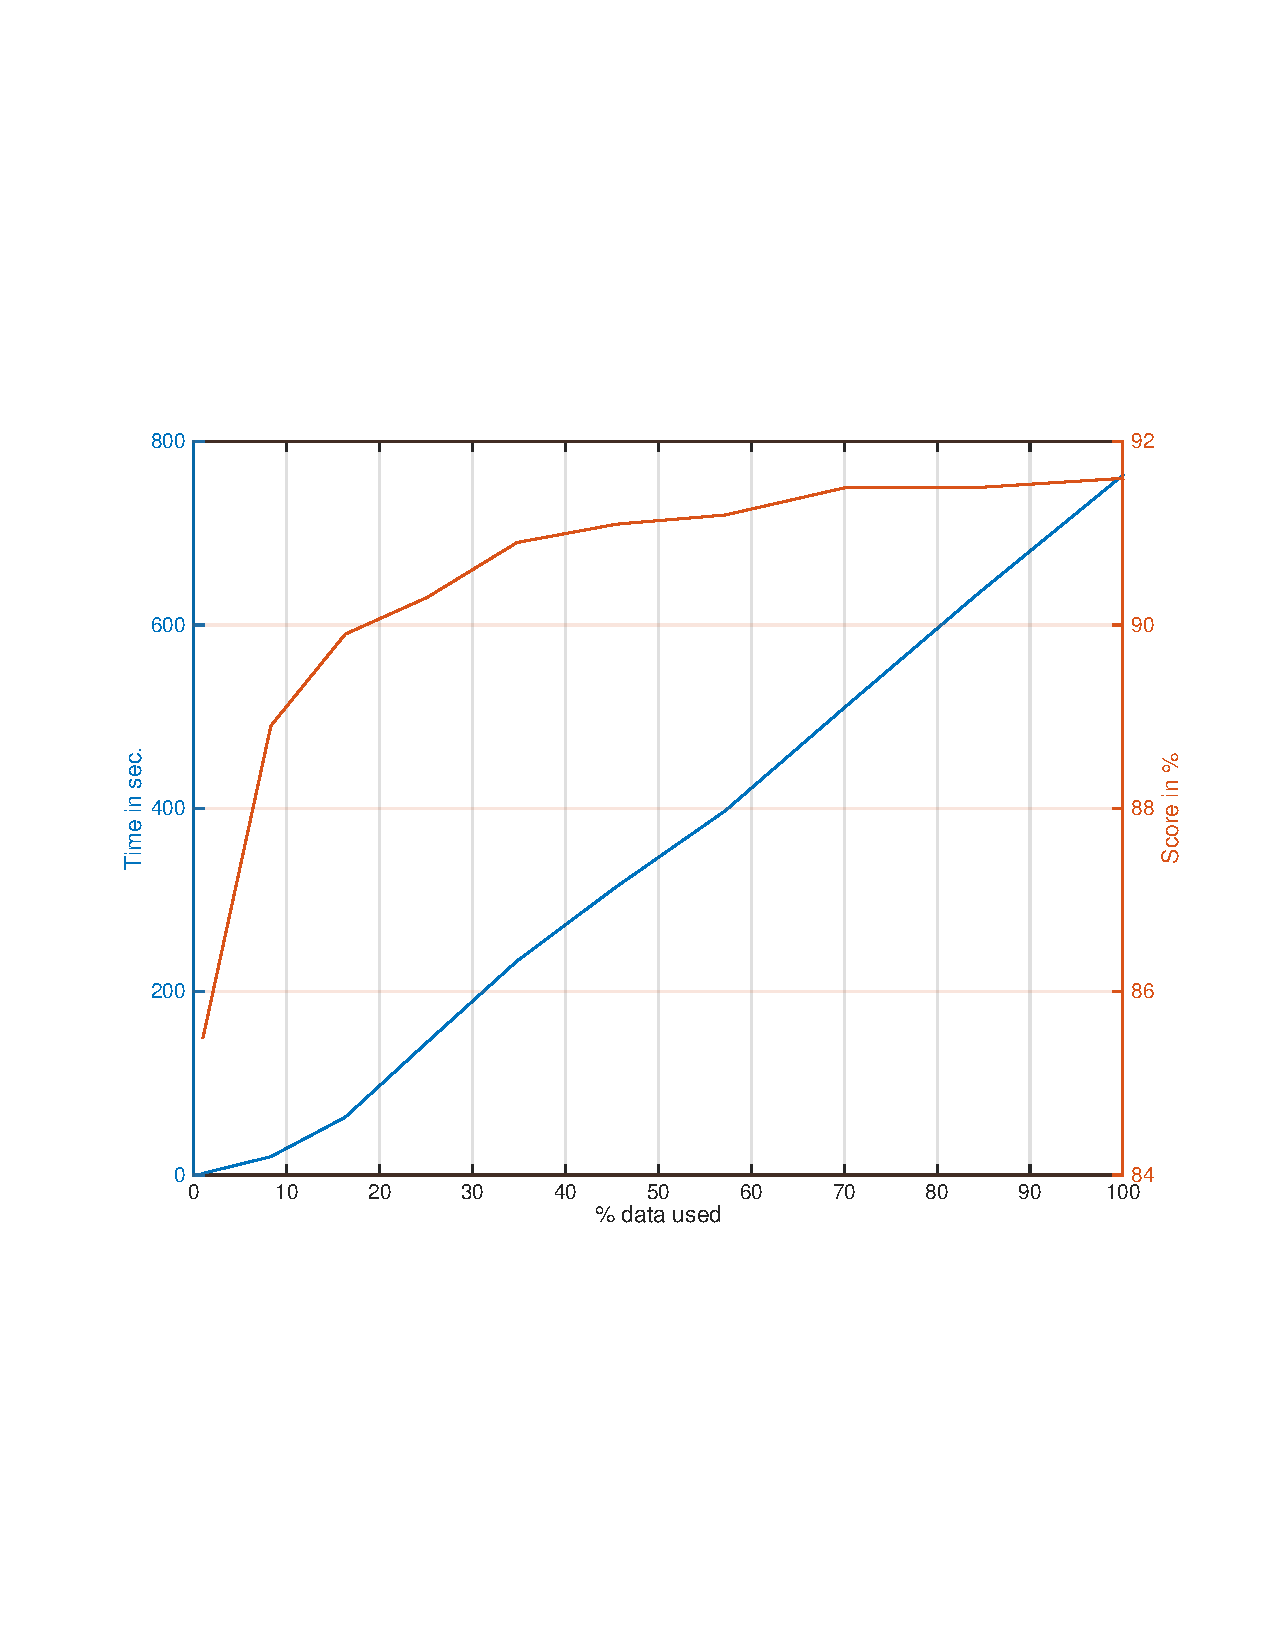
\includegraphics[trim=50 200 35 205,clip,width=\linewidth]{figures/lr_mnist.pdf}
  \caption{Logistic regression/MNIST}
  \label{sampledata1}
\end{subfigure}%
\begin{subfigure}{.45\textwidth}
  \centering
  \includegraphics[trim=50 200 35 205,clip,width=\linewidth]{figures/rf_mnist.pdf}
  \caption{Random forest/MNIST}
  \label{sampledata2}
\end{subfigure}
\begin{subfigure}{.45\textwidth}
  \centering
  \includegraphics[trim=50 200 35 205,clip,width=\linewidth]{figures/lr_synth.pdf}
  \caption{Logistic regression/synthetic data}
  \label{sampledata3}
\end{subfigure}
\begin{subfigure}{.45\textwidth}
  \centering
  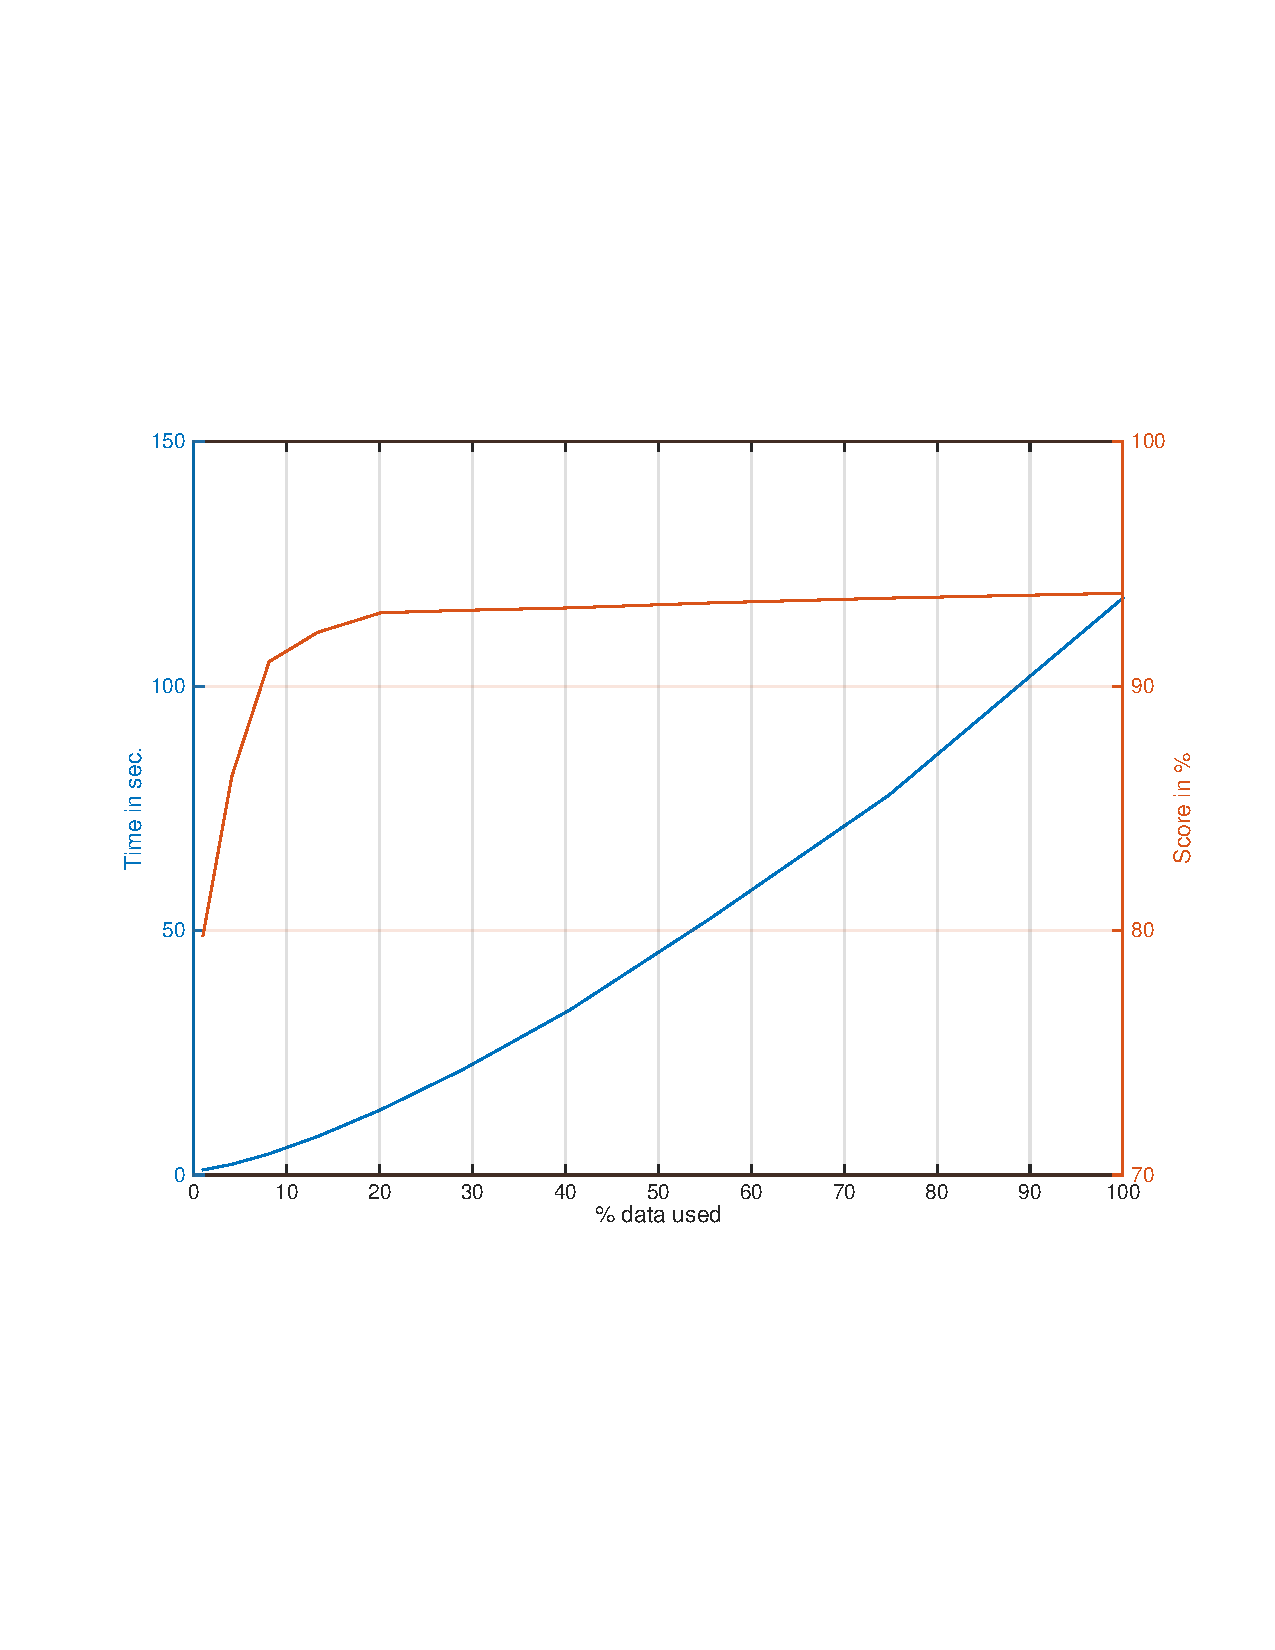
\includegraphics[trim=50 200 35 205,clip,width=\linewidth]{figures/rf_synth.pdf}
  \caption{Random forest/synthetic data}
  \label{sampledata4}
\end{subfigure}
\caption{Sample data plotting time and score against the proportion of data used}
\label{sampledata}
\end{figure}




Figure \ref{sampledata} show the results of collecting performance data, varying the percentage of data used. The four plots show the result of running random forests with 128 trees and logistic regression on the MNIST dataset and a synthetic dataset with 5000 samples and 500 features.

In all four figures, the runtime, shown in blue, exhibits linear growth as the amount of data increases. Although the runtime of random forest is $\mathcal{O}(n log n)$ instead of linear in the amount of data, we've found that in practice, it is still modelled well by a linear kernel. As runtime values shown in Figure \ref{sampledata3} are substantially lower, the values are noisier than in the other graphs, which is to be expected. 

The score (shown in red) for all four combinations of algorithms and datasets exhibits rapid growth in the beginning before levelling off. We model these curves with the exponential mixture kernel described in the next section.


\begin{figure}
\centering
\begin{subfigure}{.33\textwidth}
  \centering
  \includegraphics[trim=50 200 35 205,clip,width=\linewidth]{figures/2d_sample_data1.pdf}
  \caption{}
  \label{2d_1}
\end{subfigure}%
\begin{subfigure}{.33\textwidth}
  \centering
  \includegraphics[trim=50 200 35 205,clip,width=\linewidth]{figures/2d_sample_data2.pdf}
  \caption{}
  \label{2d_2}
\end{subfigure}
\begin{subfigure}{.33\textwidth}
  \centering
  \includegraphics[trim=50 200 35 205,clip,width=\linewidth]{figures/2d_sample_data3.pdf}
  \caption{}
  \label{2d_3}
\end{subfigure}
\caption{Three different perspectives on the same score data}
\label{2d}
\end{figure}


Figure \ref{2d} shows a plot of random forests score data for two approximation parameters. The $x$-axis shows the number of decision trees, the $y$-axis the percentage of data used. The shape of the plot suggests a multiplicative relationship between the two parameters.


\section{The Exponential Mixture Kernel}

Based on the results shown in the previous section, we implemented a kernel to model the exponential behaviour of classification accuracy. Following \cite{2014arXiv1406.3896S}, we define the kernel as

\begin{align}
\kappa(x,x') &= \int_{0}^{\infty} e^{-\lambda x}e^{-\lambda x'}\mu(d\lambda)\\
&= \int_{0}^{\infty} e^{-\lambda(x+x')}\mu(d\lambda)
\end{align}



with $\mu$ being a mixing measure\footnote{We use $\mu$ instead of $\psi$ to denote the mixing measure to avoid confusion with the $\psi$ parameter to the gamma function explained below} that weighs the $e^{-\lambda(x+x')}$ term. Note that this is not a stationary kernel as $\kappa(x, x') \neq \kappa(x + \tau, x' + \tau)$. This conforms to our prior that moving further away from the origin, the value of $\kappa$ should decrease.

Again following \cite{2014arXiv1406.3896S}, we choose a gamma distribution as $\mu$ which leads to an analytic solution to the integral:
\begin{align}
\kappa(x, x') &= \int_0^{\infty} e^{-\lambda(x+x')}\frac{\beta^\alpha}{\Gamma(\alpha)}\lambda^{\alpha -1}e^{-\lambda\beta} d\lambda\\
&=\frac{\beta^\alpha}{\Gamma(\alpha)}\int_0^\infty e^{-\lambda(x+x'+\beta)}\lambda^{\alpha-1}d\lambda\\
&=\frac{\beta^\alpha}{(x+x'+\beta)^\alpha}
\end{align}

Diverging from \cite{2014arXiv1406.3896S}, we reparameterise the gamma distribution with
\begin{equation}
\psi = \mathbb{E}(x) = \frac{\alpha}{\beta}
\end{equation}
and
\begin{align}
\xi &= \frac{Var(x)}{\mathbb{E}^2 (x)} = \frac{\alpha}{\beta^2} \cdot \frac{\beta^2}{\alpha^2}\\
&= \frac{1}{\alpha}
\end{align}

\begin{figure}
\centering
\begin{subfigure}{.5\textwidth}
  \centering
  \includegraphics[trim=80 190 70 190,clip,width=0.95\linewidth]{figures/gamma_psi.pdf}
  \caption{Varying $\psi$, $\xi$ fixed at 1.1}
  \label{gammapsi}
\end{subfigure}%
\begin{subfigure}{.5\textwidth}
  \centering
  \includegraphics[trim=80 190 70 190,clip,width=0.95\linewidth]{figures/gamma_xi.pdf}
  \caption{Varying $\xi$, $\psi$ fixed at 1.1}
  \label{gammaxi}
\end{subfigure}
\caption{Varying the parameters to the reparameterised $\Gamma$-distribution}
\label{gammadist}
\end{figure}


Figure \ref{gammadist} show how the distribution changes as $\psi$ and $\xi$ are varied. Note how the distributions Figure \ref{gammapsi} have the same shape with a different mean while the shape parameter $\xi$, shown in Figure \ref{gammaxi}, changes the shape of the distribution.

After reparameterisation, the term for our kernel becomes
\begin{equation}
\kappa(x, x') = \frac{\frac{1}{\psi\xi}^{\frac{1}{\xi}}}{(x+x'+\frac{1}{\psi\xi})^{\frac{1}{\xi}}}
\end{equation}

\begin{figure}
\centering

  \centering
  \includegraphics[trim=80 190 70 190,clip,width=.6\linewidth]{figures/expmix_psi1_xi1.pdf}
  \caption{Functions drawn from an exponential mixture kernel}
  \label{expmix11}
\end{figure}

Figure \ref{expmix11} shows functions drawn from the exponential mixture kernel. Note how these functions decay to zero as $y$ grows.

The score functions we encounter, shown in the previous section do not normally decay to zero, instead they plateau at values between zero and one. To model this effect, we add a constant function to our exponential mixture kernel as described in the Background chapter.

To model multi-dimensional data with multiple approximation parameters, we model every input dimension with a separate exponential mixture kernel and multiply these kernels together, adding a constant kernel to this product for the reason described in the previous paragraph. To model each dimension with its own kernel, we use GPML's \texttt{covMask} utility kernel that allows masking out arbitrary input dimensions.

\section{Selecting Kernel Hyperparameters} 


To achieve a good fit of a Gaussian process to a given set of data points, one needs to find appropriate values for the hyperparameters to its covariance function. There two main ways to do so are marginalisation and optimisation. For reasons explained in the Evaluation chapter, we implement both of these methods in our project.

GPML includes an optimisation function called \texttt{minimize} that is meant to be used to optimise kernel hyperparameters. It relies on gradient information, which we implemented for the exponential mixture kernel. We were, however, not able to successfully optimise the hyperparameters to our kernel with this function as the optimisation would terminate after a very small number of steps having moved only slightly from the initial values without having found a minimum. We suspect the reason for this to be numerical instability that creates small amounts of noise and creates tiny local minima that the optimiser is unable to escape from. 

Figure \ref{nlmlopt} shows a plot of a marginal likelihood function for data drawn from a Gaussian process prior that we tried to optimise with GPML's \texttt{minimize}. Clearly, this is not a difficult function to optimise in principle.

\begin{figure}
\centering
  \centering
  \includegraphics[trim=60 190 70 190,clip,width=.6\linewidth]{figures/nlml_opt.pdf}
  \caption{The negative log marginal likelihood of an exponential mixture kernel as a function of $\psi$}
  \label{nlmlopt}
\end{figure}

After failing to optimise the hyperparameters to our kernel using the optimisation function included with GPML, we decided to implement a sampling method which does not suffer from the same problems as optimisation. After successfully implementing sampling, we also decided to write our own optimisation routine for reasons of speed and ease of use. Both methods are described in detail in the remainder of this section. An evaluation of the two methods applied to our data can be found in the Evaluation chapter.

\subsection{Sampling}
One approach to hyperparameter selection is the Bayesian approach of integrating out the hyperparameters $\theta$. Recall that the marginal likelihood given data $\mathcal{D}$ and hyperparameters $\theta$ is defined as

\begin{equation}
p(\mathbf{y}|\mathcal{D}, \theta) = \int p(\mathbf{y}|f, \mathcal{D}, \theta)p(f|\mathcal{D}, \theta) df
\end{equation}

We can marginalise out $\theta$ from the marginal likelihood:

\begin{equation}
p(\mathbf{y}|\mathcal{D}) = \int p(\mathbf{y}|\mathcal{D}, \theta)p(\theta|\mathcal{D}) d\theta
\end{equation}

This integral does not have an analytic solution and, as such, must be approximated by sampling from $p(\theta|\mathcal{D})$ and calculating

\begin{equation}
p(\mathbf{y}|\mathcal{D}) \approx \sum p(\mathbf{y}|\mathcal{D}, \theta)p(\theta|\mathcal{D}) \Delta\theta
\end{equation}

% TODO MAYBE explain what sampling is ("sample from distribution")

The main advantage of sampling the hyperparameters is that it does not suffer from overfitting given that the samples are successfully drawn from the posterior distribution. Its major drawback is that it is computationally more expensive than optimisation methods. Implementation wise, sampling also takes more effort than optimisation, as the result of the computations the program executes have to be correctly averaged over.

\subsubsection{Slice sampling}

Slice sampling \cite{MacKay:2002:ITI:971143, neal2003} is a Markov Chain Monte Carlo (MCMC) sampling method. Sampling methods of this type generate samples by constructing a Markov chain that converges to the posterior distribution. The main advantage of slice sampling over other MCMC sampling methods is that it does not require careful tuning of its parameters which makes it particularly easy to use. 

The general outline of slice sampling given a distribution $f$ from which we want to sample is as follows. We start at a point $x$ and evaluate $y = f(x)$. From the interval $(0, y)$, we uniformly draw a value $u$, the height of the slice that gives slice sampling its name. The next step is to span an interval $(x_l, x_r)$ around $x$. We then draw $x'$ uniformly from this interval and calculate $y' = f(x')$. If $y' > u$, we return $x'$ as a sample. Otherwise we narrow the interval $(x_l, x_r)$ by setting $x'$ to be the new endpoint of the interval on the side of $x$ on which $x'$ falls.

Figure \ref{slsamp} shows slice sampling after the height $u$ of the slice has been chosen, the interval $(x_l, x_r)$ has been created and an $x'$ has been drawn from that interval. As $f(x')$ is less than $u$, the next step of execution will shrink the interval by setting $x_r$ to $x'$.

\begin{figure}
\centering
  \includegraphics[trim=0 0 0 0,clip,width=\textwidth]{figures/slice_sampling.pdf}
  \caption{Slice sampling}
  \label{slsamp}
\end{figure}




\subsection{Optimisation}

Another approach to find suitable hyperparameters is to optimise the marginal likelihood of the model with respect to its hyperparameters:

\begin{equation}
p_{\text{opt}}(\mathbf{y}|\mathcal{D}) = \argmax_\theta p(\mathbf{y}|\mathcal{D}, \theta)
\end{equation}


This has the advantage of being substantially faster than sampling. It is also easier to implement, as it returns one set of hyperparameters that can be used to make predictions instead of multiple samples that have to be correctly averaged over. The disadvantage of optimisation is that it is prone to overfitting by choosing one optimum in cases where multiple viable optima exist. We describe situations in which we encountered this problem in the Evaluation chapter, comparing it with the results of slice sampling.

After inspecting the marginal likelihood functions of our sample data in Matlab, we concluded they are not functions that are inherently difficult to optimise and decided to implement our own optimisation routine. As we had already successfully sampled hyperparameters using slice sampling as described above, we implemented an optimisation method that works similarly to how slice sampling draws samples. The first version of this algorithm is shown below as Algorithm \ref{opti1}.


\begin{algorithm}
\begin{algorithmic}[1]
\Procedure{Optimise}{$f,x,iterations=100,width=1$}
\State $y\gets f(x),\ D\gets \Call{get\_dimensions}{x}$
\For{$i\gets 1, iterations$}
\For{$dim\gets \Call{permute}{D}$}\Comment{Iterate over all dimensions}
\State $x_l, x_r, x'\gets x$\Comment{$x_l,\ x_r$ span interval, $x'$ falls inside}
\State $r\gets \Call{Uniform}{0, 1}$
\State $x_l(dim)\gets x(dim) - r * width$
\State $x_r(dim)\gets x(dim) + (1 - r) * width$
\For{$j\gets 1, 15$}
\State $x'(dim)\gets \Call{Uniform}{x_r(dim), x_l(dim)}$
\State $y' = f(x')$
\If{$y' < y$}
\State $y\gets y',\ x(dim) = x'(dim)$\Comment{New optimum}
\Break
\EndIf
\If{$x'(dim) > x(dim)$}
\State $x_r(dim) = x'(dim)$\Comment{Narrow interval from the right}
\ElsIf{$x'(dim < x(dim)$}
\State $x_l(dim) = x'(dim)$\Comment{Narrow interval from the left}
\EndIf
\EndFor
\EndFor
\EndFor
\EndProcedure
\end{algorithmic}
\caption{First version of our custom optimisation routine}
\label{opti1}
\end{algorithm}

This optimisation algorithm starts at a given $x$ and optimises by iterating over the input dimensions, spanning up an interval around $x$ for every iteration. Inside of these iterations, it selects points $x'$ at random from the interval. If $f(x')$ is smaller than the current minimum, it continues to the next loop iteration, otherwise it narrows the interval either from the left or the right, depending on the side of $x$ on which $x'$ falls.

Given sufficient data to fit to, this algorithm is able to find suitable hyperparameters to the exponential mixture kernel reliably. If it is used to fit a GP to a small number of points (five or less), it often selects hyperparameters such that the covariance matrix is not positive semidefinite and Cholesky decomposition fails. We catch these errors by wrapping every evaluation of $f$ in a \texttt{try ... catch} block. 

While testing this algorithm, we found an effective method to handle these errors to be rerunning the algorithm multiple times and selecting the result with the highest marginal likelihood. This also alleviates the issue of local optima which we discuss in detail in the Evaluation chapter. The code to achieve this is shown as Algorithm \ref{optiwrap}.

\begin{algorithm}
\begin{algorithmic}[1]
\Procedure{Optimise\_with\_restarts}{$f,x,restarts=5$}
\State $X \gets [\ ],\ Y \gets [\ ]$
\For{$i\gets 1, restarts$}
\State $x'\gets \Call{Optimise}{f, x}$
\State $y'\gets f(x')$
\State $\Call{append}{X, x'}$
\State $\Call{append}{Y, y'}$
\EndFor
\State $i\gets \Call{MinIndex}{Y}$
\State \textbf{return} $X(i)$
\EndProcedure
\end{algorithmic}
\caption{Rerunning the optimiser}
\label{optiwrap}
\end{algorithm}

While this updated algorithm produces adequate results, it takes substantially longer than the original version. A final change we therefore added was to terminate the optimisation routine early if the value of $y$ only changes minimally over five iterations. This condition is met during almost all optimisations and often drastically cuts short the time that our algorithm needs.

One shortcoming of this optimisation routine is that all its steps have to be axis aligned. If the gradient of the function being optimised at $x$ is not aligned with any axis, this causes the optimiser to make very small steps along multiple axes. A superior approach would be to directly move along the gradients, which are available to us. This would not be hard to implement because gradient information is available for our kernel. As our current algorithm already performs to a high standard, we did not investigate this potential improvement further.

% TODO cite henning optimisation paper


\chapter{Scheduling} 
\label{ch:scheduling}
\textit{This chapter describes the schedulers developed during the course of this project. It firsts gives a high level overview of the system architecture before describing the details of each of the schedulers.}

\section{System Architecture}

\subsection{High Level Architecture}
\begin{figure}[p]
    \centerline{\includegraphics[trim=40 90 35 90,clip,scale=0.8]{figures/architecture4.pdf}}
  \caption{High level architecture for one scheduler, shown after three iterations. Data is shown in green, machine learning algorithm in red and the scheduler in blue. Circled numbers refer to notes in the text.}
    \label{architecture}
\end{figure}


Our system is designed in a two tiered fashion. Tier 1 creates models of the data using learning algorithms that are parameterised with approximation parameters. The training time and score of these models makes up the input to tier 2. This second layer first creates meta-models of the time and score of the models in tier 1. These meta-models are then used by the scheduler to select the algorithm and approximation parameters for the next iteration and the process is repeated.

% TODO JAMES how to justify this?
In the implemented program for this project, we focus on the two algorithms described in the Background chapter, random forests and logistic regression. The approximation parameter we use is the percentage of the available data given to the learning algorithm to train.

Figure \ref{architecture} shows this architecture diagrammatically for one scheduler after three iterations. In tier 1, the dataset \raisebox{.5pt}{\textcircled{\raisebox{-.9pt} {1}}} is used as input for all model creation. The learning process is parameterised by the learning algorithm and the approximation parameters to the algorithm \raisebox{.5pt}{\textcircled{\raisebox{-.9pt} {2}}}. The runtime time and score for every iteration are saved \raisebox{.5pt}{\textcircled{\raisebox{-.9pt} {3}}} separately for every algorithm.

% TODO explain how there are multiple acquisition functions, maximum of all of them is selected
In tier 2, this performance data is used to train Gaussian processes \raisebox{.5pt}{\textcircled{\raisebox{-.9pt} {4}}}, two each for every algorithm. These Gaussian processes model the time and the score of the algorithms as the approximation parameter is varied. These meta-models form the input to the scheduler \raisebox{.5pt}{\textcircled{\raisebox{-.9pt} {5}}} that uses them to make a decision on an algorithm/approximation parameter combination for the next iteration \raisebox{.5pt}{\textcircled{\raisebox{-.9pt} {6}}}.

\begin{figure}[ht]
\begin{lstlisting}[language=Python]
while True:
   scheduler.decide() # Tier 2 (scheduling)
   if scheduler.decision:
      scheduler.execute() # Tier 1
      scheduler.model() # Tier 2 (modelling)
\end{lstlisting}
\caption{The main loop}
\label{mainloop}
\end{figure}


Note how both tiers execute machine learning algorithms (coloured in red) on data (coloured in green) and how the result of the algorithms in the first tier form the dataset for the Gaussian Processes. The main loop of our program is shown, slightly simplified, in Figure \ref{mainloop}. When executing, the program switches back and forth between the two tiers: it executes an algorithm with a given set of approximation parameters, builds a new model that includes the performance during this execution. The scheduler then decides which algorithm/approximation parameter combination to run next and the system returns to the first step.

\begin{figure}[p]
    \centerline{\includegraphics[trim=70 120 50 120,clip,scale=0.475]{figures/system_example.pdf}}
  \caption{The program running with three schedulers}
    \label{systemexample}
\end{figure}

Figure \ref{systemexample} shows the program running with three schedulers. Rows one to three are each one instance of the architecture depicted in Figure \ref{architecture}; the plot in row four compares the performance of the three schedulers. For the three running instances, the first column shows runtime information. Logistic regression data is shown in blue while random forests data is shown in red. The dots represent recorded data points, the blue line shows the mean of the model that predicts runtime while the filled area is twice the standard deviation of the model, showing the uncertainty the model has. The scheduler shown in row one does not require models to make decisions and only shows the recorded data points. For schedulers that operate on time budgets, this plot also shows how much time is currently remaining by drawing a black line at the time threshold.

The plot in the second column shows the score data and model in the same way the time information is drawn. Additionally, for schedulers that model time and score (the second and third in the example), the acquisition functions for both algorithm is shown as dashed line. The precise shape of these functions depends on the strategy the scheduler uses to make decision. 

The third row contains plots of the time against the score function as a point cloud for logistic regression (blue) and random forests (red). These point clouds are created by drawing 100 points each from the time and score model and plotting one against the other. Again, these plots are only computed for schedulers that model performance data.





\subsection{Directory Structure of the Code}

The directory of the project contains the following subdirectories:
\begin{itemize}
\item \textbf{data/}: This directory contains the datasets in \texttt{data/raw\_arffs/} and data generated by the sample data generation scripts is stored. When creating plots based on this data, the results are also written to this folder
\item \textbf{figs/}: Every diagram our system displayes is automatically also saved to this directory
\item \textbf{report}/: This folder is where the source file and diagrams for this document are stored
\item \textbf{src/}: This directory holds all the source code for our project. It contains \texttt{main.py}, the main code file and two subdirectories, \texttt{src/data\_handling/} and \texttt{src/matlab/} which contain Python and Matlab code respectively
\item \textbf{var/}: This folder is used to store temporary files that are used to exchange data between Python and Matlab code
\end{itemize}



\subsection{Interoperability between Python and Matlab}
Choosing Matlab to implement the performance modelling code and Python to implement the other parts of our system made it necessary to devise a method of transferring data between these two parts of the program. During the initial planning stage, we intended to write all parts of the system in Python but the advantages of GPML such as level of documentation and ease of use later outweighed the disadvantages of having to deal with process interoperability.

To start the program, the \texttt{main.py} file is executed. This file then calls the Matlab script that contains modelling code whenever it has collected new data and needs to update one of its performance models. Data is transferred between the Python and the Matlab scripts by writing it to \texttt{json} files\footnote{JSON is a widespread data format similar to XML.} in the \texttt{var/} directory.  Before the Matlab script is executed, \texttt{main.py} writes the recorded performances of the algorithm for which it has just updated its data to \texttt{var/scheduler\_data.json}. This file contains a JSON object with the fields \texttt{x\_percent\_data}, \texttt{y\_times} and \texttt{y\_scores} which hold the data collected so far.

Once it has finished modelling, the Matlab script writes the models to \texttt{var/models.json} and terminates. This file contains an array of model objects. These models are represented as 100 equally spaced data points between 0\% and 100 \% of available data. They each have an \texttt{m} and an \texttt{sd} field for the mean and standard deviation respectively. This file is then read by \texttt{main.py} and the old models are overwritten with the updated ones.


\section{Implemented Schedulers}
\begin{figure}
    \centerline{\includegraphics[trim=55 70 35 55,clip,width=\linewidth]{figures/scheduler_inheritance.pdf}}
  \caption{The inheritance structure of the implemented schedulers. Abstract schedulers are shown in grey}
    \label{schedulerinheritance}
\end{figure}

Every scheduler is implemented in a separate class of which there are nine in total. There are three abstract scheduler classes that implement functionality shared between two or more schedulers while the other six implement scheduling strategies that can be used to schedule data collection. The inheritance structure of the scheduler classes is shown in Figure \ref{schedulerinheritance}. In this section, we describe each scheduler's functionality before comparing and evaluating them in the Evaluation chapter.

\subsection{\texttt{\textit{Scheduler}}}
This is the base class that all schedulers inherit from. It defines a framework of functionality that all schedulers share. Besides drawing routines and code to write performance and read model data, this class contains the following methods:

\begin{itemize}
\item \texttt{\_\_init\_\_}: the class constructer initialises a number of properties, including the \texttt{self.data} property which holds an array of learning performances for each algorithm
\item \texttt{decide}: this is a virtual method that is called to decide on the next algorithm/approximation parameter combination to be evaluated. It sets the \texttt{self.decision} property of the scheduler object. If the scheduler is done, either due to having finished optimising or because its time budget has been used up, this property is set to \texttt{None}
\item \texttt{execute}: this method executes the decision made by the \texttt{decide} method and adds the new time and score to the \texttt{self.data} property
\item \texttt{model}: this function updates the model for the algorithm for which data was collected during the last execution of the \texttt{execute} method. It reads the value of the \texttt{self.decision} property to determine the algorithm and is to be called after \texttt{execute} finishes
\end{itemize}


\subsection{\texttt{FixedSequenceScheduler}}
% TODO different name for this, not "decision list"
\texttt{FixedSequenceScheduler} is the simplest of all the scheduling strategies implemented. Its constructor takes a sequence of data percentage values and computes the cartesian product of the learning algorithms and this sequence and saves this decision list. When its \texttt{decide} method is called, it writes the next element of the decision list into \texttt{self.decision}, cycling through algorithms and executing the fixed sequence of data percentage values. Once it has executed every algorithm/data percentage combination, the scheduler terminates.

This scheduler is unique among the schedulers in not requiring a model of runtime and score. Its evaluation sequence is set during initialisation and it does not rely on predictions to decide which learning algorithm/approximation parameter combination to try next.



\subsection{\texttt{\textit{ProbablisticScheduler}}}

This is the base class of all schedulers that make probabilistic decisions using an acquisition function as described in the Bayesian Optimisation section of the Background chapter. Its constructor expects an array that contains values for the approximation parameter used during an initial burn-in phase. During this phase, the schedulers collect the initial performance data and to not create model.

This scheduler has a virtual class method \texttt{a} that takes a time and score model (expressed as arrays of mean and standard deviation) and calculates the acquisition function. If slice sampling was used to integrate out the hyperparameters to the exponential mixture kernel, \texttt{\textit{ProbablisticScheduler}} is responsible for calling \texttt{a} as many times as there are samples and averaging over these acquisition functions. Time and score model samples are taken independently which allows us to randomly pair one time and one score model per iteration.

\subsection{\texttt{ProbabilityOfImprovementScheduler}}
This is the simplest concrete probabilistic scheduler. It implements the probability of improvement heuristic for Bayesian optimisation. As mentioned in the Background chapter, this is not an optimal scheduling strategy. It is, however, still included for purposes of comparison.

This scheduler truncates its acquisition function at the maximum $x$ value for each algorithm and only considers percentage of data values that are strictly greater than its current maximum. This encodes the assumption that using more data can never produce a model worse than the current best.

\subsection{\texttt{ExpectedImprovementScheduler}}
\texttt{ExpectedImprovementScheduler} implements the Expected improvement heuristics for Bayesian optimisation. Like the \texttt{ProbabilityOfImprovementScheduler}, it truncates its acquisition function and only considers using more data than before for subsequent execution of the learning algorithms.

\subsection{\texttt{ExpectedImprovementPerTimeScheduler}}
This scheduler inherits from the \texttt{ExpectedImprovementScheduler} and differs from it only by dividing the expected improvement by the mean of the time model. This biases it towards faster executions of the learning algorithms, even if the improvement over the current best is not as large as slower executions.

\subsection{\texttt{\textit{TimedScheduler}}}
\texttt{\textit{TimedScheduler}} is the base class of the two schedulers that operate on a finite time budget. It inherits from \texttt{\textit{ProbablisticScheduler}} and includes functionality to keep track of the remaining time and add a line to the time plot to show how much time is left.

\subsection{\texttt{ExpectedImprovementTimesProbOfSuccessScheduler}}
This scheduler inherits from both the \texttt{\textit{TimedScheduler}} and the \texttt{ExpectedImprovementScheduler}. To compute its acquisition function, it multiplies the expected improvement with the probability of successfully finishing the learning process in the remaining time. The probability of success for a given $x$ value is calculated by cutting off the distributions of the time model at $x$ and computing the amount of remaining probability mass.

The constructor of \texttt{ExpectedImprovementTimesProbOfSuccessScheduler} expects a sequence of time intervals. Whenever the scheduler has used up its available time budget, the next time interval in the sequence is added to the remaining time.

\subsection{\texttt{MinimeseUncertaintyThenExploitScheduler}}
The \texttt{MinimeseUncertaintyThenExploitScheduler} inherits from \texttt{\textit{TimedScheduler}}. It has two scheduling phases and is allocated a separate time budget for each phase. In the first phase, it tries to build adequate models by reducing uncertainty. Its acquisition function during this phase is calculated as the score model standard deviation divided by the time it takes to evaluate the function at the point under consideration.% This behaviour is similar to the \texttt{ExpectedImprovementPerTimeScheduler} using.

After using up the time allotted for exploration, this scheduler uses the second time budget to construct the best model it can within that time, using the models it constructed during the first phase.


\chapter{Evaluation}
% TODO END add "recall that"

\textit{This chapter describes the results of our project and evaluates the system we built. It also lists challenges that we faced during its development and limitations it currently has.}




\section{Datasets}
The first set of datasets we used was created synthetically using scikit-learn's \texttt{make\_classification} function. This function takes a number of parameters that define the dataset, such as the number of samples, the number of features and the number of classes and creates data according to these parameters. 

This fine grained control over the properties of the datasets was very valuable to us, as it allowed us to see how our system handles datasets of different nature. We wrote a small script\footnote{Saved at \texttt{src/data\_handling/dataset\_creator.py}} to enable us to quickly create datasets and see how logistic regression and random forests perform on subsets of these datasets.


A second set of datasets was drawn from the list of datasets that were used in the development of Auto-WEKA as mentioned in the Related Work chapter. The authors of Auto-WEKA made the datasets used to test Auto-WEKA available on their website\footnote{They can be downloaded at http://www.cs.ubc.ca/labs/beta/Projects/autoweka/datasets/}.


These datasets originally came from other sources \cite{Lichman:2013, Larochelle:2007:EED:1273496.1273556, Krizhevsky09learningmultiple} and were converted by the Auto-WEKA creators to WEKA's own data format, the Attribute-Relation File Format (\texttt{arff}). This made it very convenient for us to use these datasets as they are originally in a wide range of differing data formats and would have had to have individual import routines written for them. 

Besides converting them to the \texttt{arff} format, the authors of the Auto-WEKA paper also split them up in a training and a test set. As we described in the Implementation chapter, we implement k-fold cross-validation and therefore needed all the data in a single file. To achieve this, a small ruby script\footnote{Saved at \texttt{src/data\_handling/utils/append\_arff\_files.rb}} was written to merge the \texttt{train.arff} and \texttt{test.arff} files for each dataset. Table \ref{datasets_info} lists the names and sizes of these datasets.


\begin{table}
\centering


\begin{tabular}{|l|l|l|l|}
\hline
Dataset          & \# samples & \# features & \# classes \\ \hline\hline
Abalone          & 4177       & 8           & 28         \\ \hline
Amazon           & 1500       & 10000       & 50         \\ \hline
Car              & 1728       & 6           & 4          \\ \hline
Germancredit     & 1000       & 20          & 2          \\ \hline
Krvskp           & 3196       & 36          & 2          \\ \hline
Madelon          & 2600       & 500         & 2          \\ \hline
Semeion          & 1593       & 256         & 10         \\ \hline
Shuttle          & 58000      & 9           & 7          \\ \hline
Waveform         & 5000       & 40          & 3          \\ \hline
Winequalitywhite & 4898       & 11          & 7          \\ \hline
Yeast            & 1484       & 8           & 10         \\ \hline\hline
MNIST            & 62000      & 784         & 10         \\ \hline
%Cifar10small     & 20000      & 3072        & 10         \\ \hline
Synthetic1            & 10000       & 500           & 2         \\ \hline
Synthetic2            & 10000       & 1000           & 2         \\ \hline
Synthetic3            & 20000       & 1500           & 2         \\ \hline
Synthetic4            & 40000       & 2000           & 2         \\ \hline
\end{tabular}

\caption{Datasets used for evaluation with large datasets shown at the bottom}
\label{datasets_info}

\end{table}


While some of the datasets in this collection are entirely numerical, some have textual features while still others have a mixture of strings and numbers as features. An example of this is the \texttt{germancredit} dataset, which has a feature \texttt{credit\_history} with possible values such as \texttt{"all paid"} and \texttt{"critical/other existing credit"}. It also has a feature called \texttt{age} that is of type integer.

When using these datasets, we load the \texttt{arff} files using SciPy's \texttt{scipy.io.arff.loadarff} function. As scikit-learn expects the features to all be numerical, we convert the data using a technique called one-of-k encoding.


This encoding expands every feature of type string with $n$ possible values into $n$ boolean typed features. This means that a feature such as \texttt{other\_payment\_plans}, also taken from the \texttt{germancredit} dataset, with possible values \texttt{bank}, \texttt{stores} and \texttt{none} is converted to three separate features, \texttt{other\_payment\_plans=bank}, \texttt{other\_payment\_plans=stores} and \texttt{other\_payment\_plans=none}. For every sample in the dataset, one of these features is be set to $1$ and all others to $0$, according to the value of \texttt{other\_payment\_plans}.


\section{Model Comparison}
In this section, we assess the quality of the fits to score data our exponential mixture kernel achieves. We do so by comparing the marginal likelihoods of the models it generates to those of a kernel that encodes weaker prior knowledge about the shape of the data, the squared exponential kernel.




\subsection{In one Dimension}



\begin{table}
\centering
	\begin{tabular}{|l|l|l|l|}
\hline
Dataset          & Exp. mixture nlml & Squared exp. nlml & Bayes factor \\ \hline\hline
Abalone          & \textbf{-37.984}  & -34.138  & 3.846         \\ \hline
Amazon           & \textbf{-24.641}  & -21.769  & 2.872         \\ \hline
Car              & \textbf{-30.685}  & -25.251  & 5.434         \\ \hline
Germancredit     & \textbf{-27.806}  & -23.858  & 3.948         \\ \hline
Krvskp           & \textbf{-33.710}  & -30.226  & 3.484         \\ \hline
Madelon          & -24.786           & \textbf{-25.212} & -0.426  \\ \hline
Semeion          & \textbf{-32.969}  & -27.234  & 5.735         \\ \hline
Shuttle          & \textbf{-45.728}  & -44.317  & 1.411         \\ \hline
Waveform         & \textbf{-38.294}  & -27.317  & 10.977        \\ \hline
Winequalitywhite & \textbf{-34.842}  & -32.331  & 2.511         \\ \hline
Yeast            & -28.428           & \textbf{-28.676} & -0.248  \\ \hline\hline
MNIST            & \textbf{-46.028}  & -37.350  & 8.678         \\ \hline
Synthetic1       & \textbf{-30.107}  & -11.668  & 18.439        \\ \hline
Synthetic2       & \textbf{-24.622}  & -11.661  & 12.961        \\ \hline
Synthetic3       & \textbf{-19.479}  & -15.978  & 3.5014        \\ \hline
Synthetic4       & \textbf{-16.761}  & -7.059   & 9.702         \\ \hline
\end{tabular}

	\caption{The negative log marginal likelihoods of fitting an exponential mixture kernel and a squared exponential kernel to logistic regression score data}
\label{log_reg_fits}
\end{table}


\begin{table}
\centering
\begin{tabular}{|l|l|l|l|}
\hline
Dataset          & Exp. mixture nlml & Squared exp. nlml & Bayes factor \\ \hline\hline
Abalone          & -                 & -       & -              \\ \hline
Amazon           & \textbf{-20.737}  & -18.355 & 2.382          \\ \hline
Car              & \textbf{-27.436}  & -24.440 & 2.996          \\ \hline
Germancredit     & \textbf{-24.955}  & -23.857 & 1.098          \\ \hline
Krvskp           & \textbf{-35.775}  & -27.289 & 8.486          \\ \hline
Madelon          & \textbf{-24.589}  & -23.921 & 0.668          \\ \hline
Semeion          & \textbf{-22.272}  & -18.516 & 3.756          \\ \hline
Shuttle          & \textbf{-50.859}  & -47.183 & 3.676          \\ \hline
Waveform         & \textbf{-32.038}  & -27.309 & 4.729          \\ \hline
Winequalitywhite & \textbf{-27.074}  & -24.302 & 2.772          \\ \hline
Yeast            & \textbf{-24.474}  & -23.146 & 1.328          \\ \hline\hline
MNIST            & \textbf{-41.603}  & -30.850 & 10.753         \\ \hline
Synthetic1       & \textbf{-25.364}  & -13.954 & 11.41          \\ \hline
Synthetic2       & \textbf{-25.224}  & -14.714 & 10.511         \\ \hline
Synthetic3       & \textbf{-20.865}  & -15.708 & 5.158          \\ \hline
Synthetic4       & \textbf{-22.73}   & -10.559 & 12.171         \\ \hline
\end{tabular}
	\caption{The negative log marginal likelihoods of fitting an exponential mixture kernel and a squared exponential kernel to random forests score data}
\label{rnd_forest_fits}
\end{table}

Tables \ref{log_reg_fits} and \ref{rnd_forest_fits} show negative log marginal likelihoods  of fits to data percentage by score data for our test datasets. We compare the negative log marginal likelihoods of a squared exponential kernel with our exponential mixture kernel. As described in the Background chapter, the squared exponential kernel only encodes a smoothness prior and is commonly used as a baseline against kernels that encode stronger priors.

For the negative log marginal likelihood, smaller values indicate a better fit. To compare the marginal likelihoods for the two kernels, we compute the Bayes factor as the quotient of the two marginal likelihoods. Since our marginal likelihoods are expressed in logspace, this is equal to the difference between the values for each kernel. The Bayes factor is to be interpreted as a measure of how much better one model is than the other. Greater values for the Bayes factor are better in our case, as they express a better fit for the exponential mixture kernel.

In tables \ref{log_reg_fits} and \ref{rnd_forest_fits}, we have grouped our datasets into small and large datasets, separated by a double line. As can be seen from inspecting the tables, the Bayes factors for the large datasets are substantially larger than those for smaller datasets. This is due to the fact that the score data for small datasets tends to be much more noisy than for large datasets were learning takes a substantial amount of time.

Figure \ref{madelon_logreg_fit} shows the two fits for the madelon dataset and random forests score data with the squared exponential kernel in blue and the exponential mixture kernel in red. The data, shown as black crosses, is so noisy, that the optimiser was not able to find a sensible fit using the exponential mixture kernel.

\begin{figure}
\centering
  \includegraphics[trim=50 200 50 200,clip,frame,width=.6\textwidth]{figures/madelon_logreg_fit.pdf}
  \caption{Fits for the madelon logistic regression score data}
  \label{madelon_logreg_fit}
\end{figure}

Figure \ref{synth3_rndforest_fit} shows the two fits for the Synthetic3 dataset, where the exponential mixture kernel, again shown in red, achieves a much better fit than the squared exponential kernel. For $x$ values that lie beyond the datapoints available, the exponential mixture kernel makes confident predictions that conform to our expectation of having reached a plateau.

\begin{figure}
\centering
  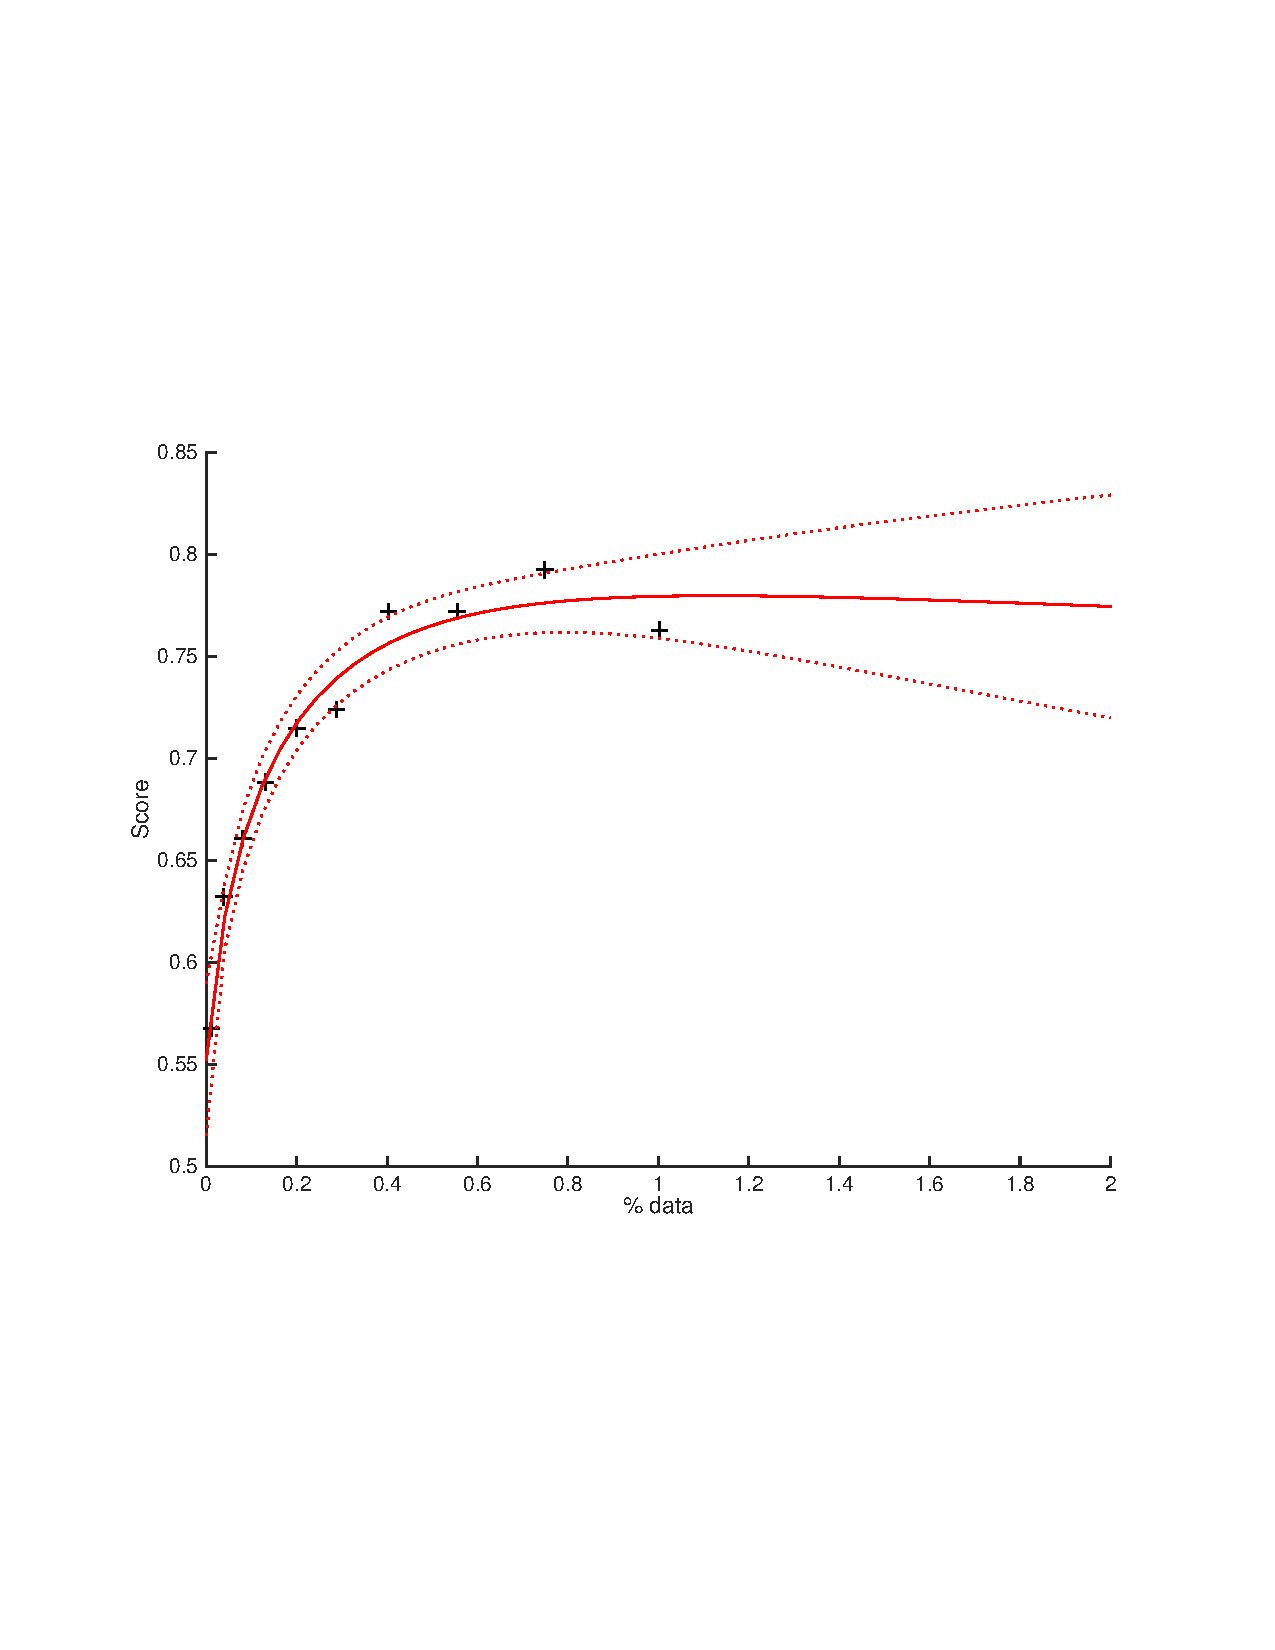
\includegraphics[trim=50 200 50 200,clip,frame,width=.6\textwidth]{figures/synth3_rndforest_fit.pdf}
  \caption{Fits for the Synthetic3 logistic regression score data}
  \label{synth3_rndforest_fit}
\end{figure}

Our results show that the exponential mixture kernel is an appropriate choice to model the score data for large datasets where it achieves a substantially better fit than the squared exponential kernel. We don't consider the weaker performance of our kernel on score data for small datasets a significant weakness. The reason for this is that the problems that we attempt to make a contribution towards solving with this problem, approximateness trade-offs when learning, do not arise when there is little data. In these cases, it is normally feasible to simply use all the available data, as doing so will only take very little time.

\subsection{In two Dimensions}


\section{The Exponential Mixture Kernel}

\subsection{Hyperparameter Selection}

We generally found both of the methods we use for hyperparameter selection, sampling and optimisation, to return satisfactory results. As is in its nature, however, optimisation is prone to overfitting. This happens when there are multiple likely interpretations of the data reflected in multiple optima of the marginal likelihood. Optimisation can only choose one of these optima and becomes overfitting in one particular interpretation of the data.

This is an issue especially in the early phases of data collection after a few iterations when only little data was available. We addressed this problem by increasing the number of data points collected during the burn-in phase. As the subsets used in this phase are a small percentage of the whole dataset, this only adds marginally to the time spent on burn-in.

Although this solved the issue of overfitting on too little data, sampling hyperparameters still proved more robust and less likely to return models that clash with the expectations that we had looking at the data. Figures \ref{kernel_issues_big1} and \ref{kernel_issues3} show cases of optimisation with such results.

\begin{figure}
\centering
\begin{subfigure}{.45\textwidth}
  \centering
  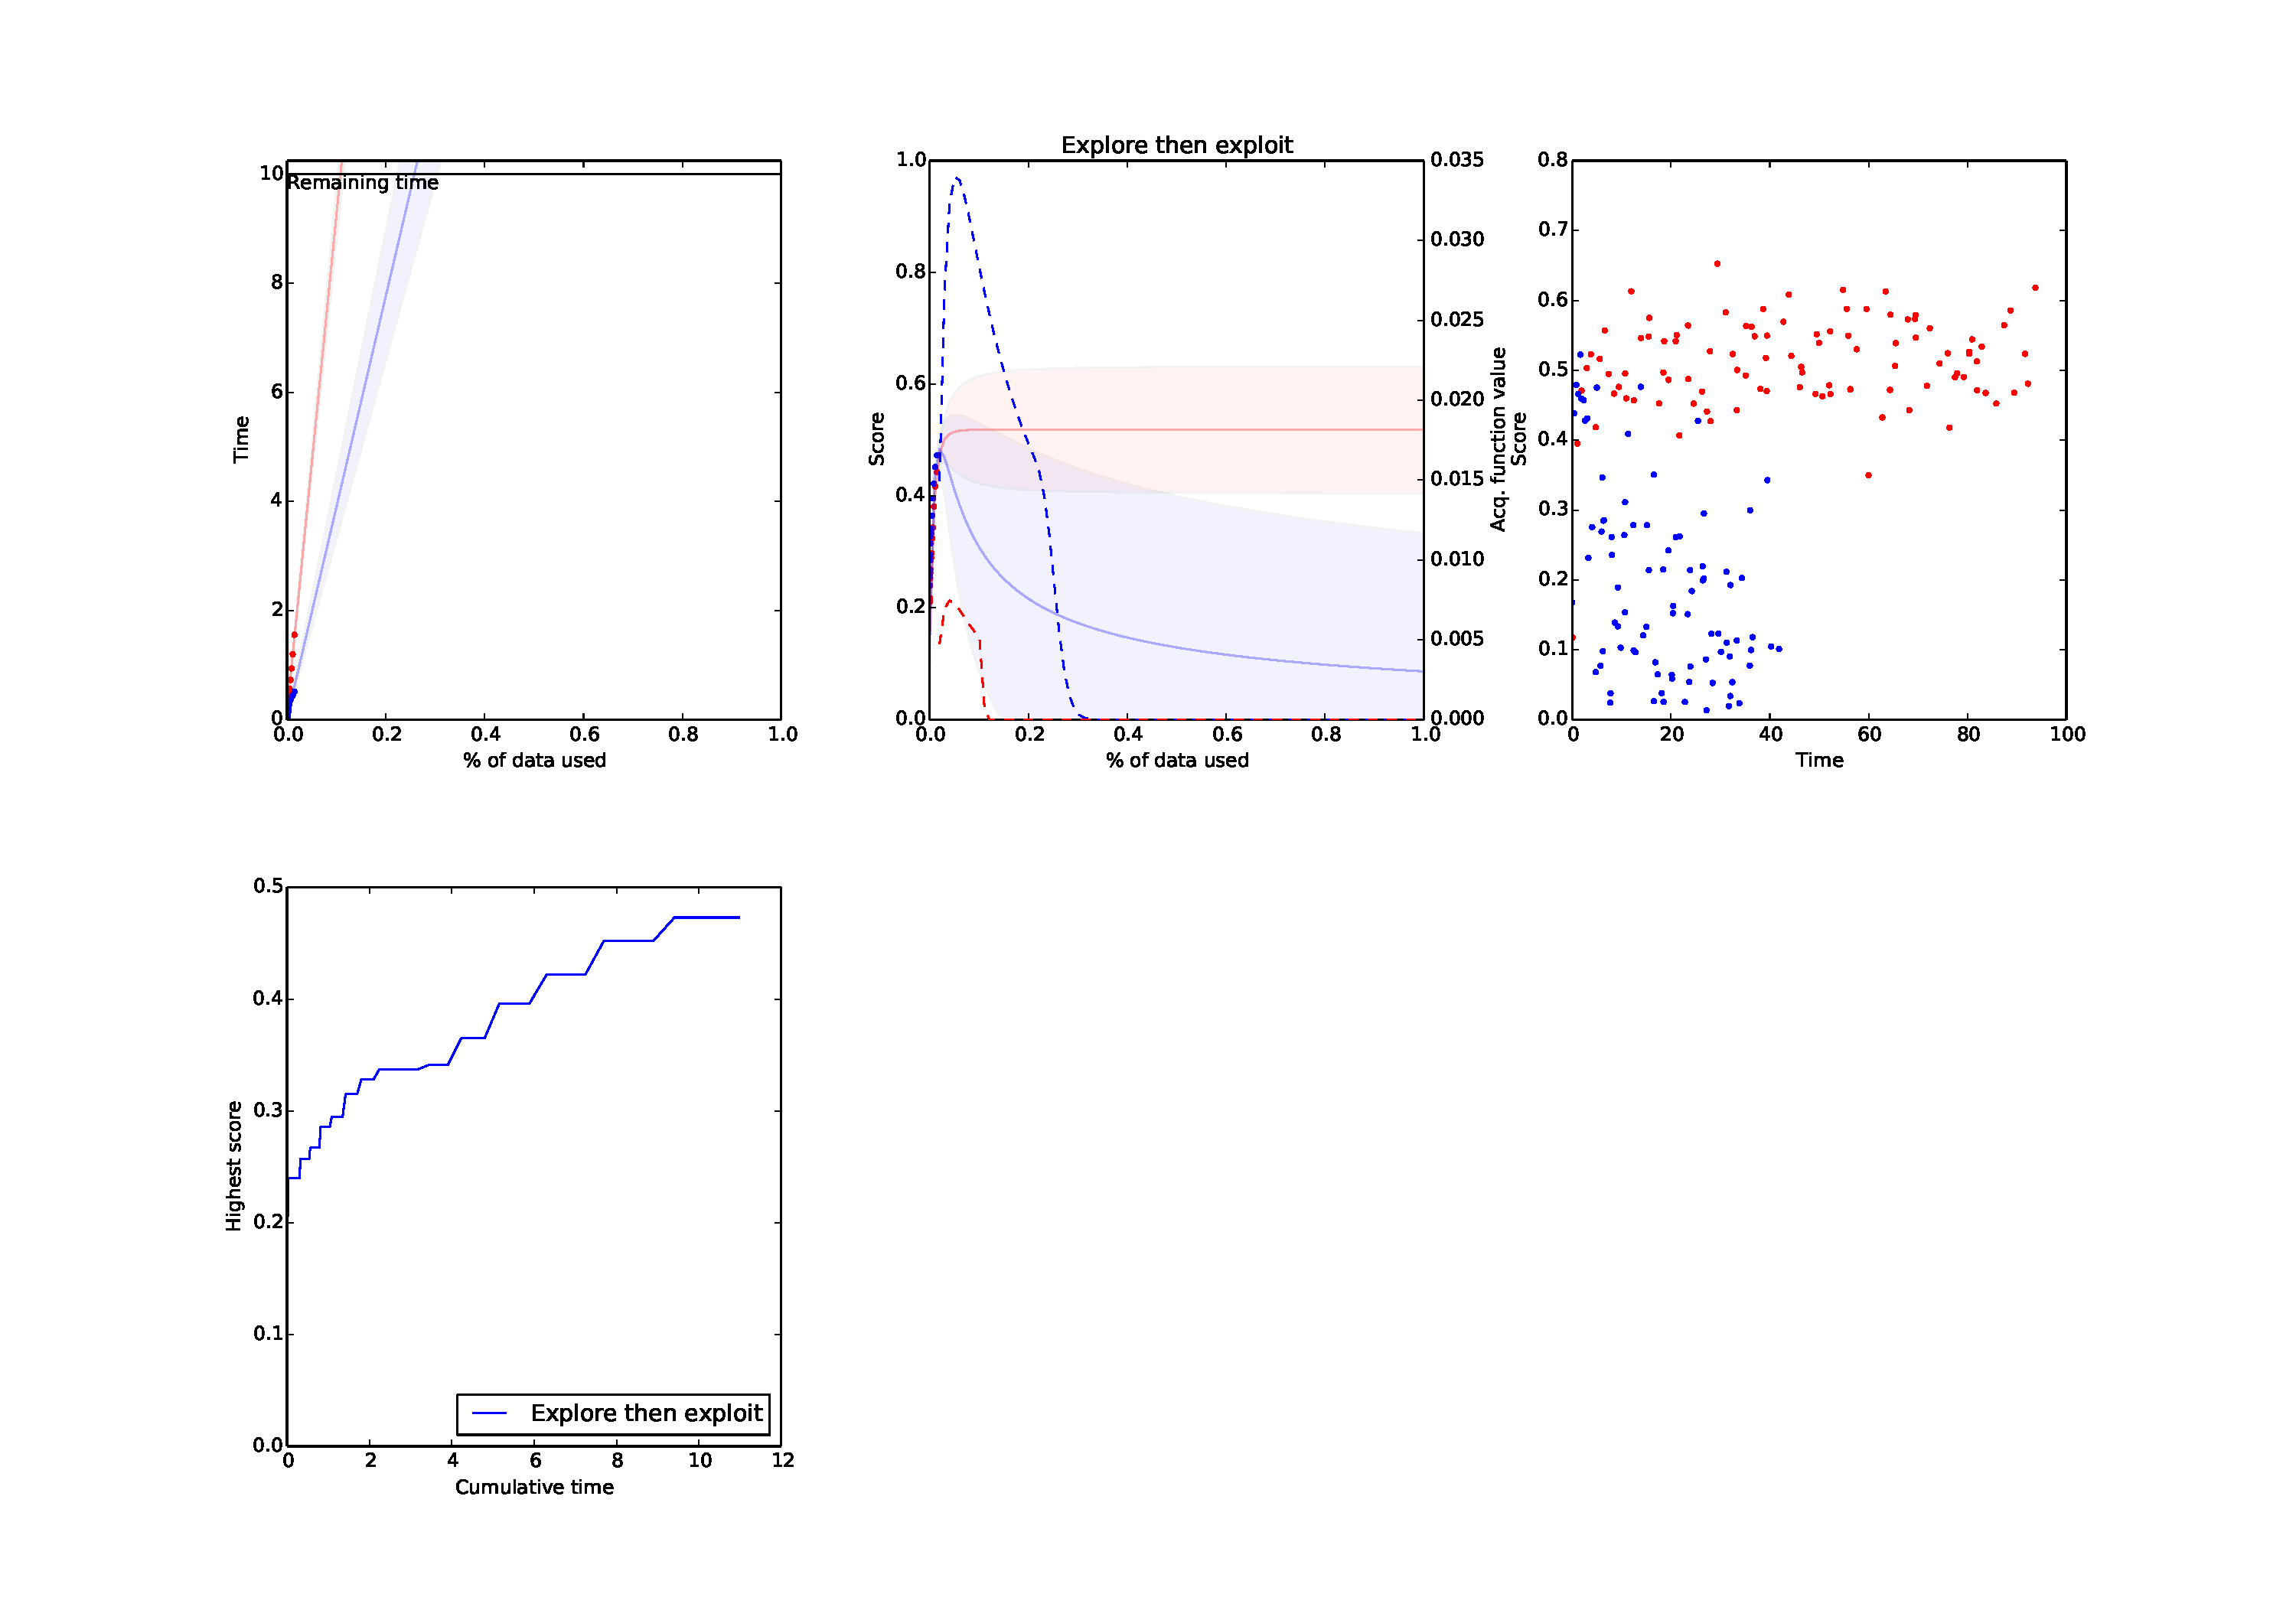
\includegraphics[trim=540 520 493 80,clip,width=\textwidth]{figures/kernel_issues1.pdf}
\caption{The blue mean grows in the wrong direction}
  \label{kernel_issues1}
\end{subfigure}%
\begin{subfigure}{.45\textwidth}
  \centering
  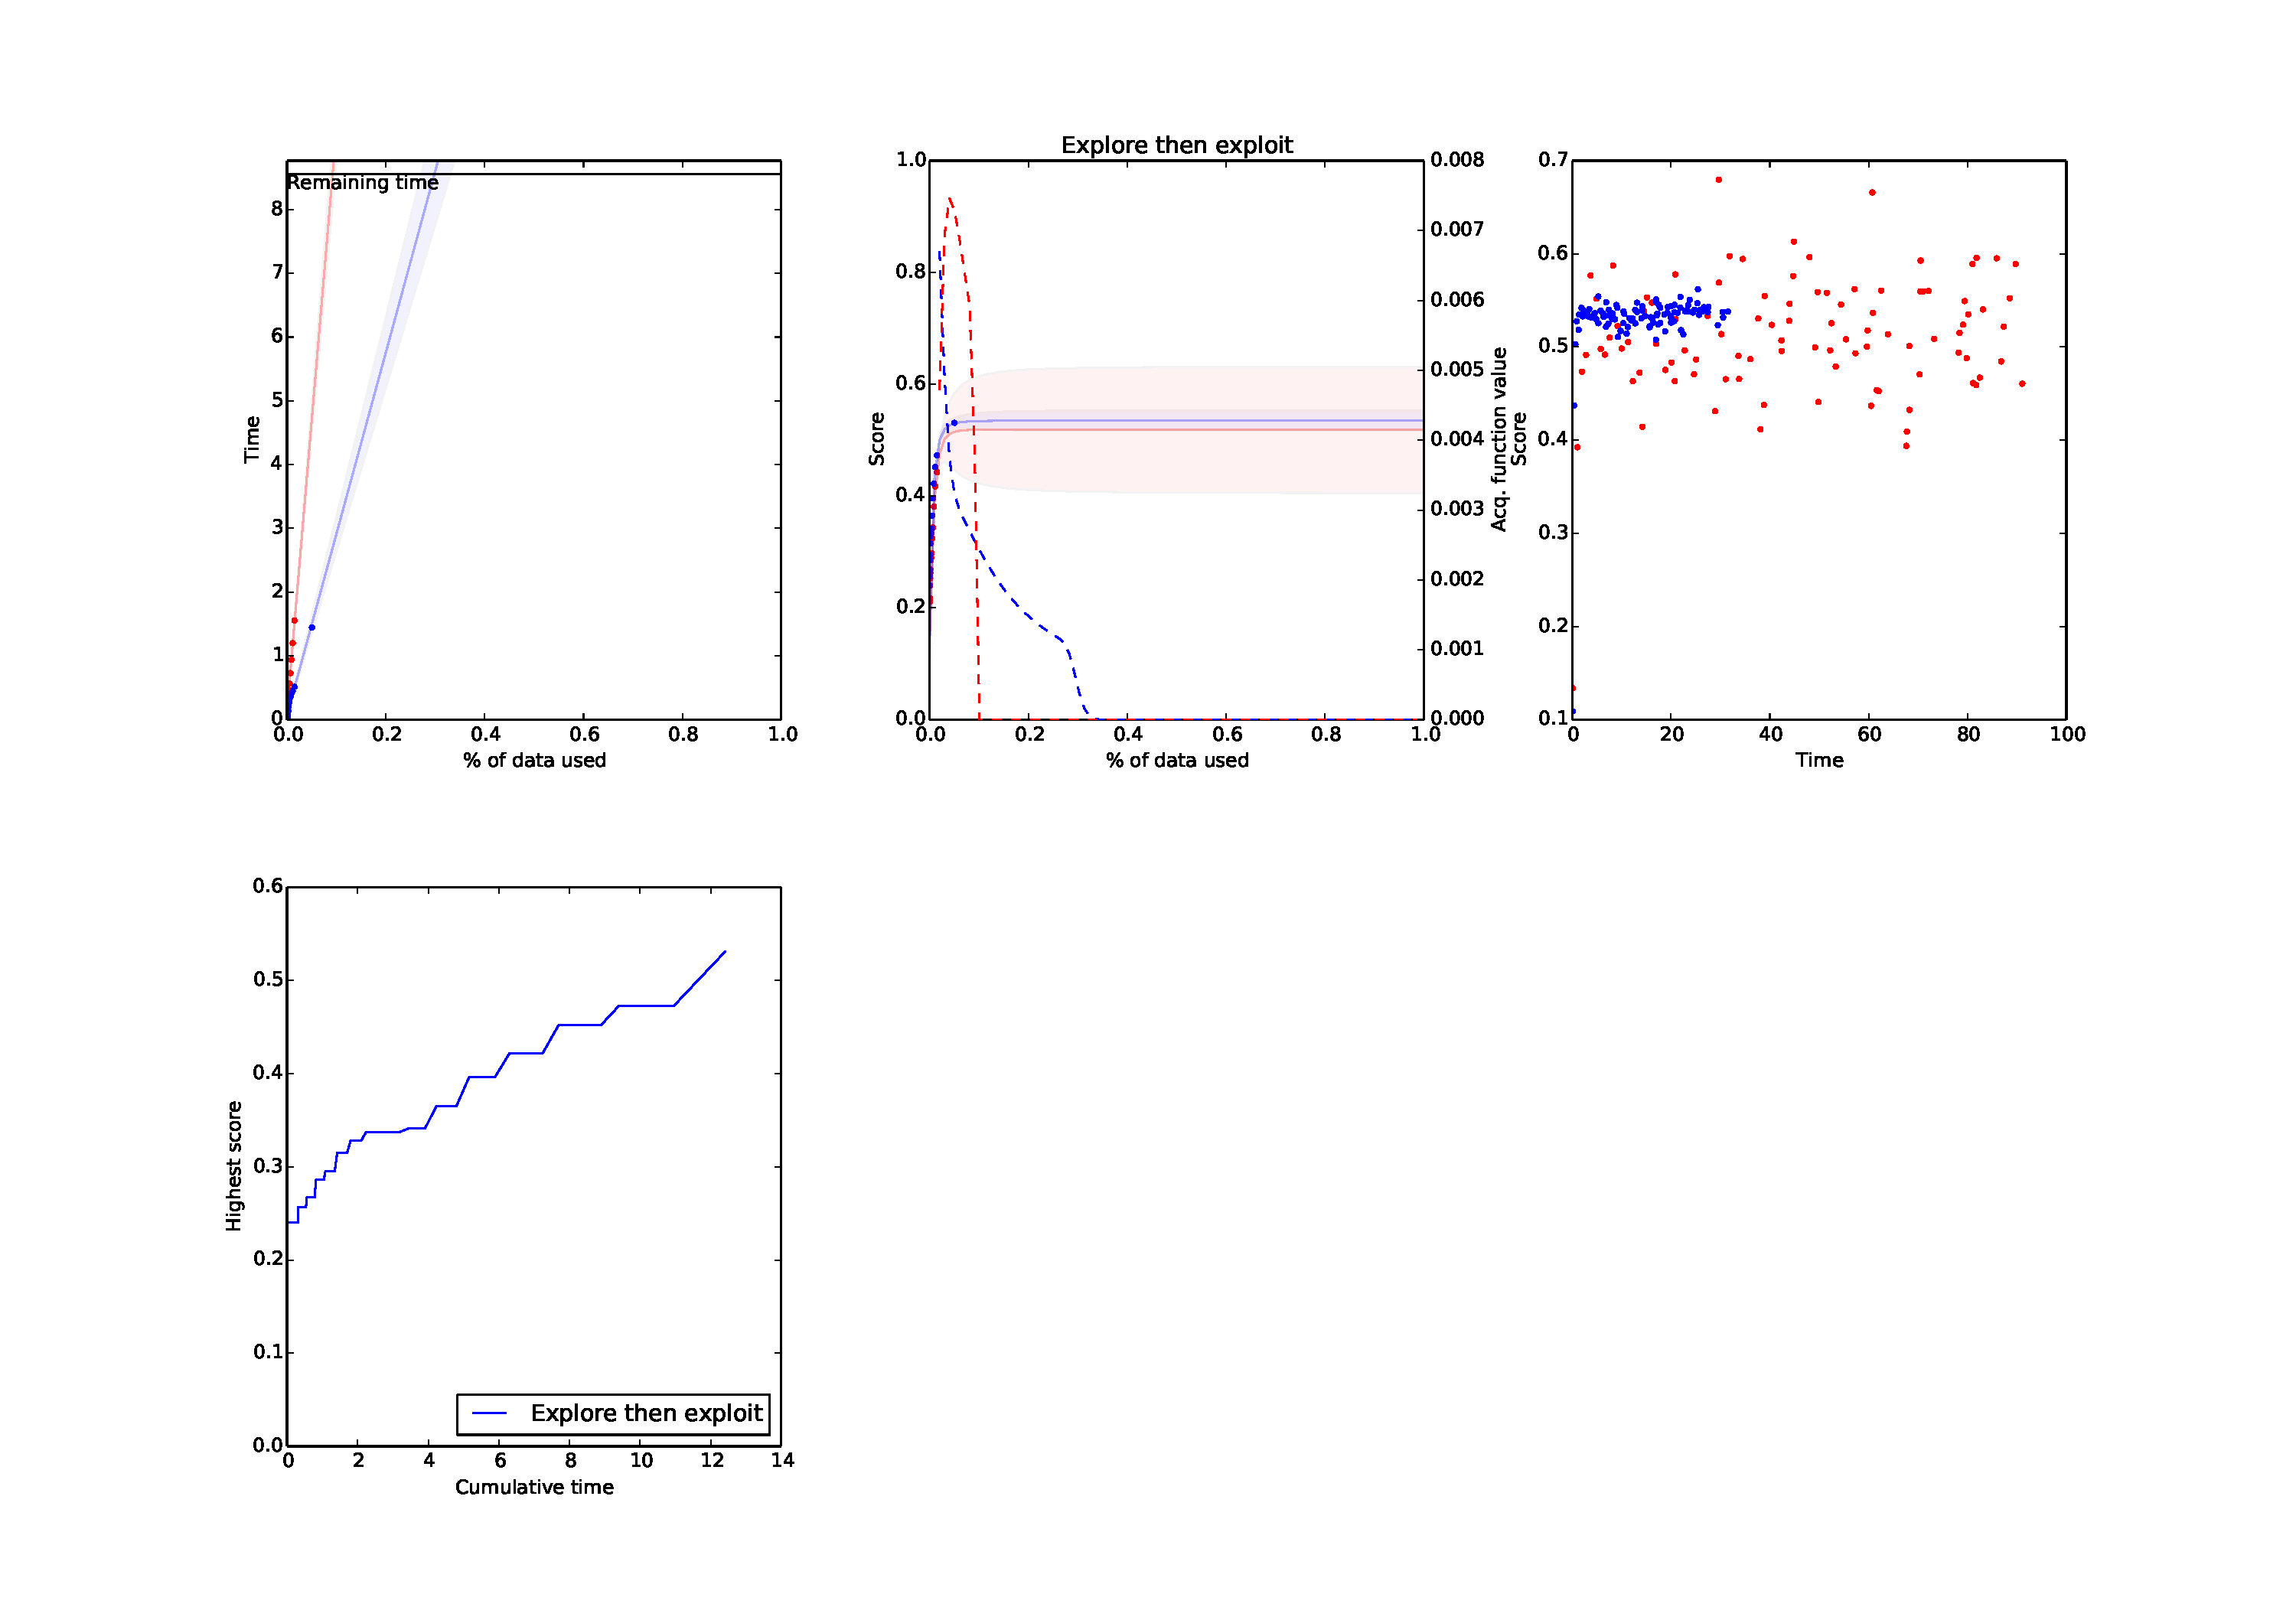
\includegraphics[trim=540 520 493 80,clip,width=\textwidth]{figures/kernel_issues2.pdf}
  \caption{Both means have a shape unlikely to be correct and the blue models' variance is too low}
  \label{kernel_issues2}
\end{subfigure}
\caption{Optimisation issues}
\label{kernel_issues_big1}
\end{figure}

\begin{figure}
\centering
  \includegraphics[trim=540 710 500 75,clip,width=\textwidth]{figures/kernel_issues3.pdf}
  \caption{The red model completely fails to model the exponential nature of the data}
  \label{kernel_issues3}
\end{figure}

As our program has to be able to handle both samples and single results returned by optimisation, we treat the result of our optimisation routine as a single sample in the routines that make use of our model. This makes it completely transparent to these routines which of the two hyperparameter selection methods were used and enables us to switch between them according to the requirements of the schedulers.

\begin{figure}
\centering
  \includegraphics[trim=540 360 493 370,clip,width=\textwidth]{figures/sampling_example.pdf}
  \caption{An example of models with sampled hyperparameters}
  \label{sampling_example}
\end{figure}

Figure \ref{sampling_example} shows models that are obtained by sampling hyperparameters. Every solid red and blue line is the mean of one model. To compute the red acquisition function for random forest, the acquisition functions for all red models are computed and averaged over. The same is done for logistic regression.

\section{Scheduling Results}

\subsection{Scheduler Behaviour}

\subsubsection{\texttt{FixedSequenceScheduler}}
\begin{figure}
\centering
  \includegraphics[trim=130 275 507 510,clip,width=\textwidth]{figures/fixed_sequence_example.pdf}
  \caption{A fixed exponential sequence}
  \label{fixedsequenceexample}
\end{figure}

Figure \ref{fixedsequenceexample} shows a \texttt{FixedSequenceScheduler} with a geometric sequence of data percentage values after about 25 iterations. In the last iteration, it trained logistic regression with about 80\% of the available data (the rightmost blue dot on both subplots) and is about to learn using random forests on the same amount of data.

This scheduler does not model performance data and does not adjust its decisions during the course of its execution.


\subsubsection{\texttt{ProbabilityOfImprovementScheduler}}
\begin{figure}
\centering
  \includegraphics[trim=530 496 510 296,clip,width=\textwidth]{figures/prob_of_imp_01.pdf}
  \caption{Probability of improvement acquisition function}
  \label{sched:probofimpr1}
\end{figure}

The \texttt{ProbabilityOfImprovementScheduler} tends to be conservative in exploring the function. Figure \ref{sched:probofimpr1} shows the score models and the acquisition functions for both algorithms as dashed lines. Although it models logistic regression to have a higher score for all $x$ values, it is less sure about how the score of this algorithm changes as $x$ grows. Consequently, it will create a random forests model next.

Although the uncertainty about the performance of random forests does not change by much for larger $x$ values, as it does for logistic regression, the probability of improvement acquisition function for random forests has its maximum at about 0.25 and decreases for larger values than that. This is due to the fact that the probability of improvement scheduler does not consider the magnitude of the increase over the current best value.

\begin{figure}
\centering

  \includegraphics[trim=530 270 507 510,clip,width=\textwidth]{figures/prob_of_imp_02.pdf}
  \caption{Probability of improvement acquisition function}
  \label{sched:probofimpr2}
\end{figure}

Figure \ref{sched:probofimpr2} shows a situation similar to the one shown in Figure \ref{sched:probofimpr1} with the difference that the uncertainty is roughly equal for both algorithms. The acquisition functions behave accordingly with the acquisition function for random forests being lower because it is less likely to improve over the current maximum $y$ which was achieved by logistic regression.

\begin{figure}
\centering
  \includegraphics[trim=530 710 493 55,clip,width=\textwidth]{figures/prob_of_imp_03.pdf}
  \caption{Probability of improvement acquisition function}
  \label{sched:probofimpr3}
\end{figure}

In Figure \ref{sched:probofimpr3}, we see the final state of a probability of improvement scheduler. The small step size in creating logistic regression models is a typical behaviour of this scheduler. 

\subsubsection{\texttt{ExpectedImprovementScheduler}}

Although the purpose of this scheduler in our program is to function as a superclass for more complex schedulers, it is nevertheless necessary to study its behaviour to understand these more complex schedulers.


Figure \ref{sched:expimpr01} shows typical acquisition functions for the \texttt{ExpectedImprovementScheduler}. Recall that the expected improvement strategy automatically balances exploration and exploitation, and that both, a high mean and a high variance increase the value of the acquisition function. Figure \ref{sched:expimpr01} demonstrates this effect: while the mean of both meta models for $x$ values greater than about 0.4 are almost equal, the expected improvement for random forests overtakes the one for logistic regression because its variance is greater.

\begin{figure}
\centering
  \includegraphics[trim=530 710 493 55,clip,width=\textwidth]{figures/expimpr01.pdf}
  \caption{Expected improvement acquisition function}
  \label{sched:expimpr01}
\end{figure}



\subsubsection{\texttt{ExpectedImprovementPerTimeScheduler}}
\begin{figure}
\centering
  \includegraphics[trim=140 710 493 55,clip,width=\textwidth]{figures/ei_by_time_1.pdf}
  \caption{Expected improvement per time performance models and acquisition function}
  \label{sched:expimprpertime01}
\end{figure}

The \texttt{ExpectedImprovementPerTimeScheduler} is a slight variation of the \texttt{ExpectedImprovementScheduler}. To calculate its acquisition function, it divides the expected improvement by the mean of the time model. Figure \ref{sched:expimprpertime01} shows the bias this scheduler has towards models that can be created quickly. Although the expected improvement increases as $x$ becomes larger, the required time also grows (shown in the left plot).

% TODO in the scheduler explanation section, mention that "success" means finishing in time
% TODO emphasize that these are the two truly new schedulers, anytime & contract
% TODO mention that some schedulers trim their acquisition functions while others dont
\subsubsection{\texttt{ExpectedImprovementTimesProbOfSuccessScheduler}}

This is one of two schedulers that expect to be given a time budget during initialisation. Figure \ref{sched:expimprpertime01} shows the state of the scheduler with one second to spend after the burn-in phase has finishd. This time limit is marked on the left plot. As can be seen on that plot, the probability that creating a random forests model with more than about 10\% of data will finish in time is extremely low. Consequently, the acquisition function for random forests is essentially flat and not visible in the right plot.

\begin{figure}
\centering
  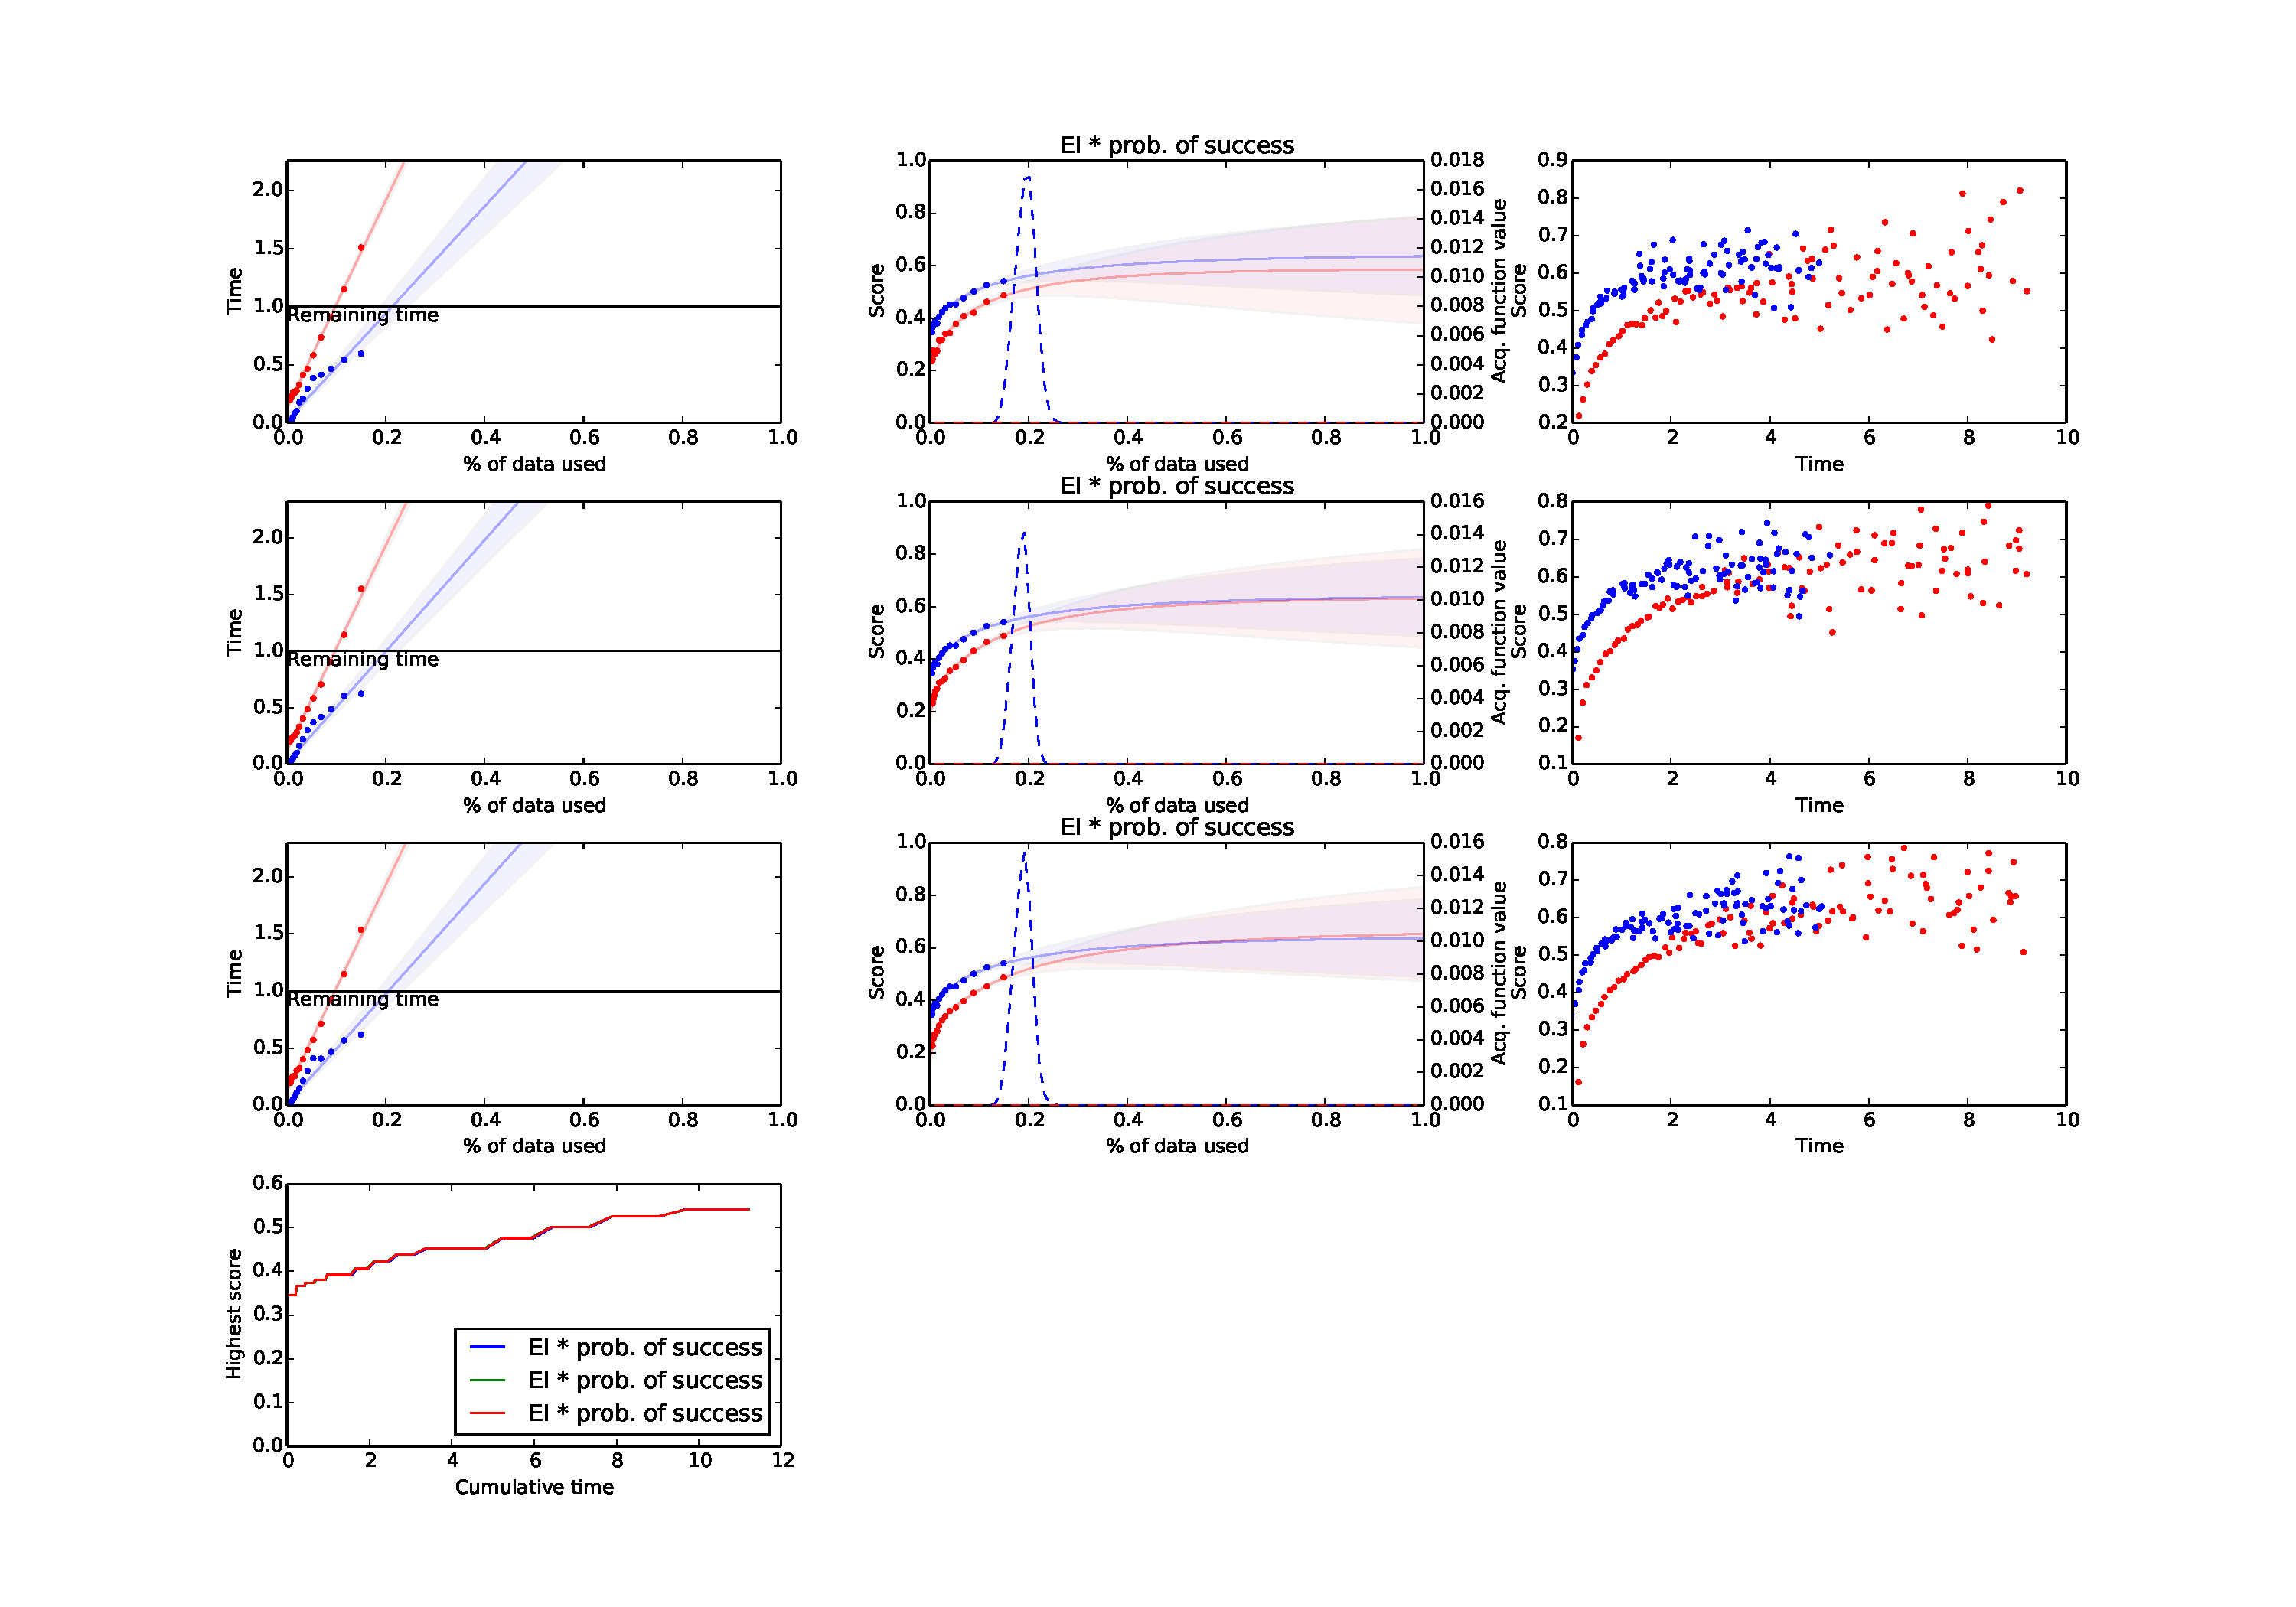
\includegraphics[trim=140 710 493 55,clip,width=\textwidth]{figures/ei_probofsuccess1.pdf}
  \caption{Expected improvement times probability of success after the burn-in period with an initial time budget of one second}
  \label{sched:expimprpertime01}
\end{figure}

The acquisition function of logistic regression algorithm with its peak around 0.2 reflects that the fact that, although the runtime of logistic regression grows slower, the time model predicts that creating a logistic regression model with 20\% of the data will take about one second. For values larger than that, the probability of success rapidly decreases.

\begin{figure}
\centering
  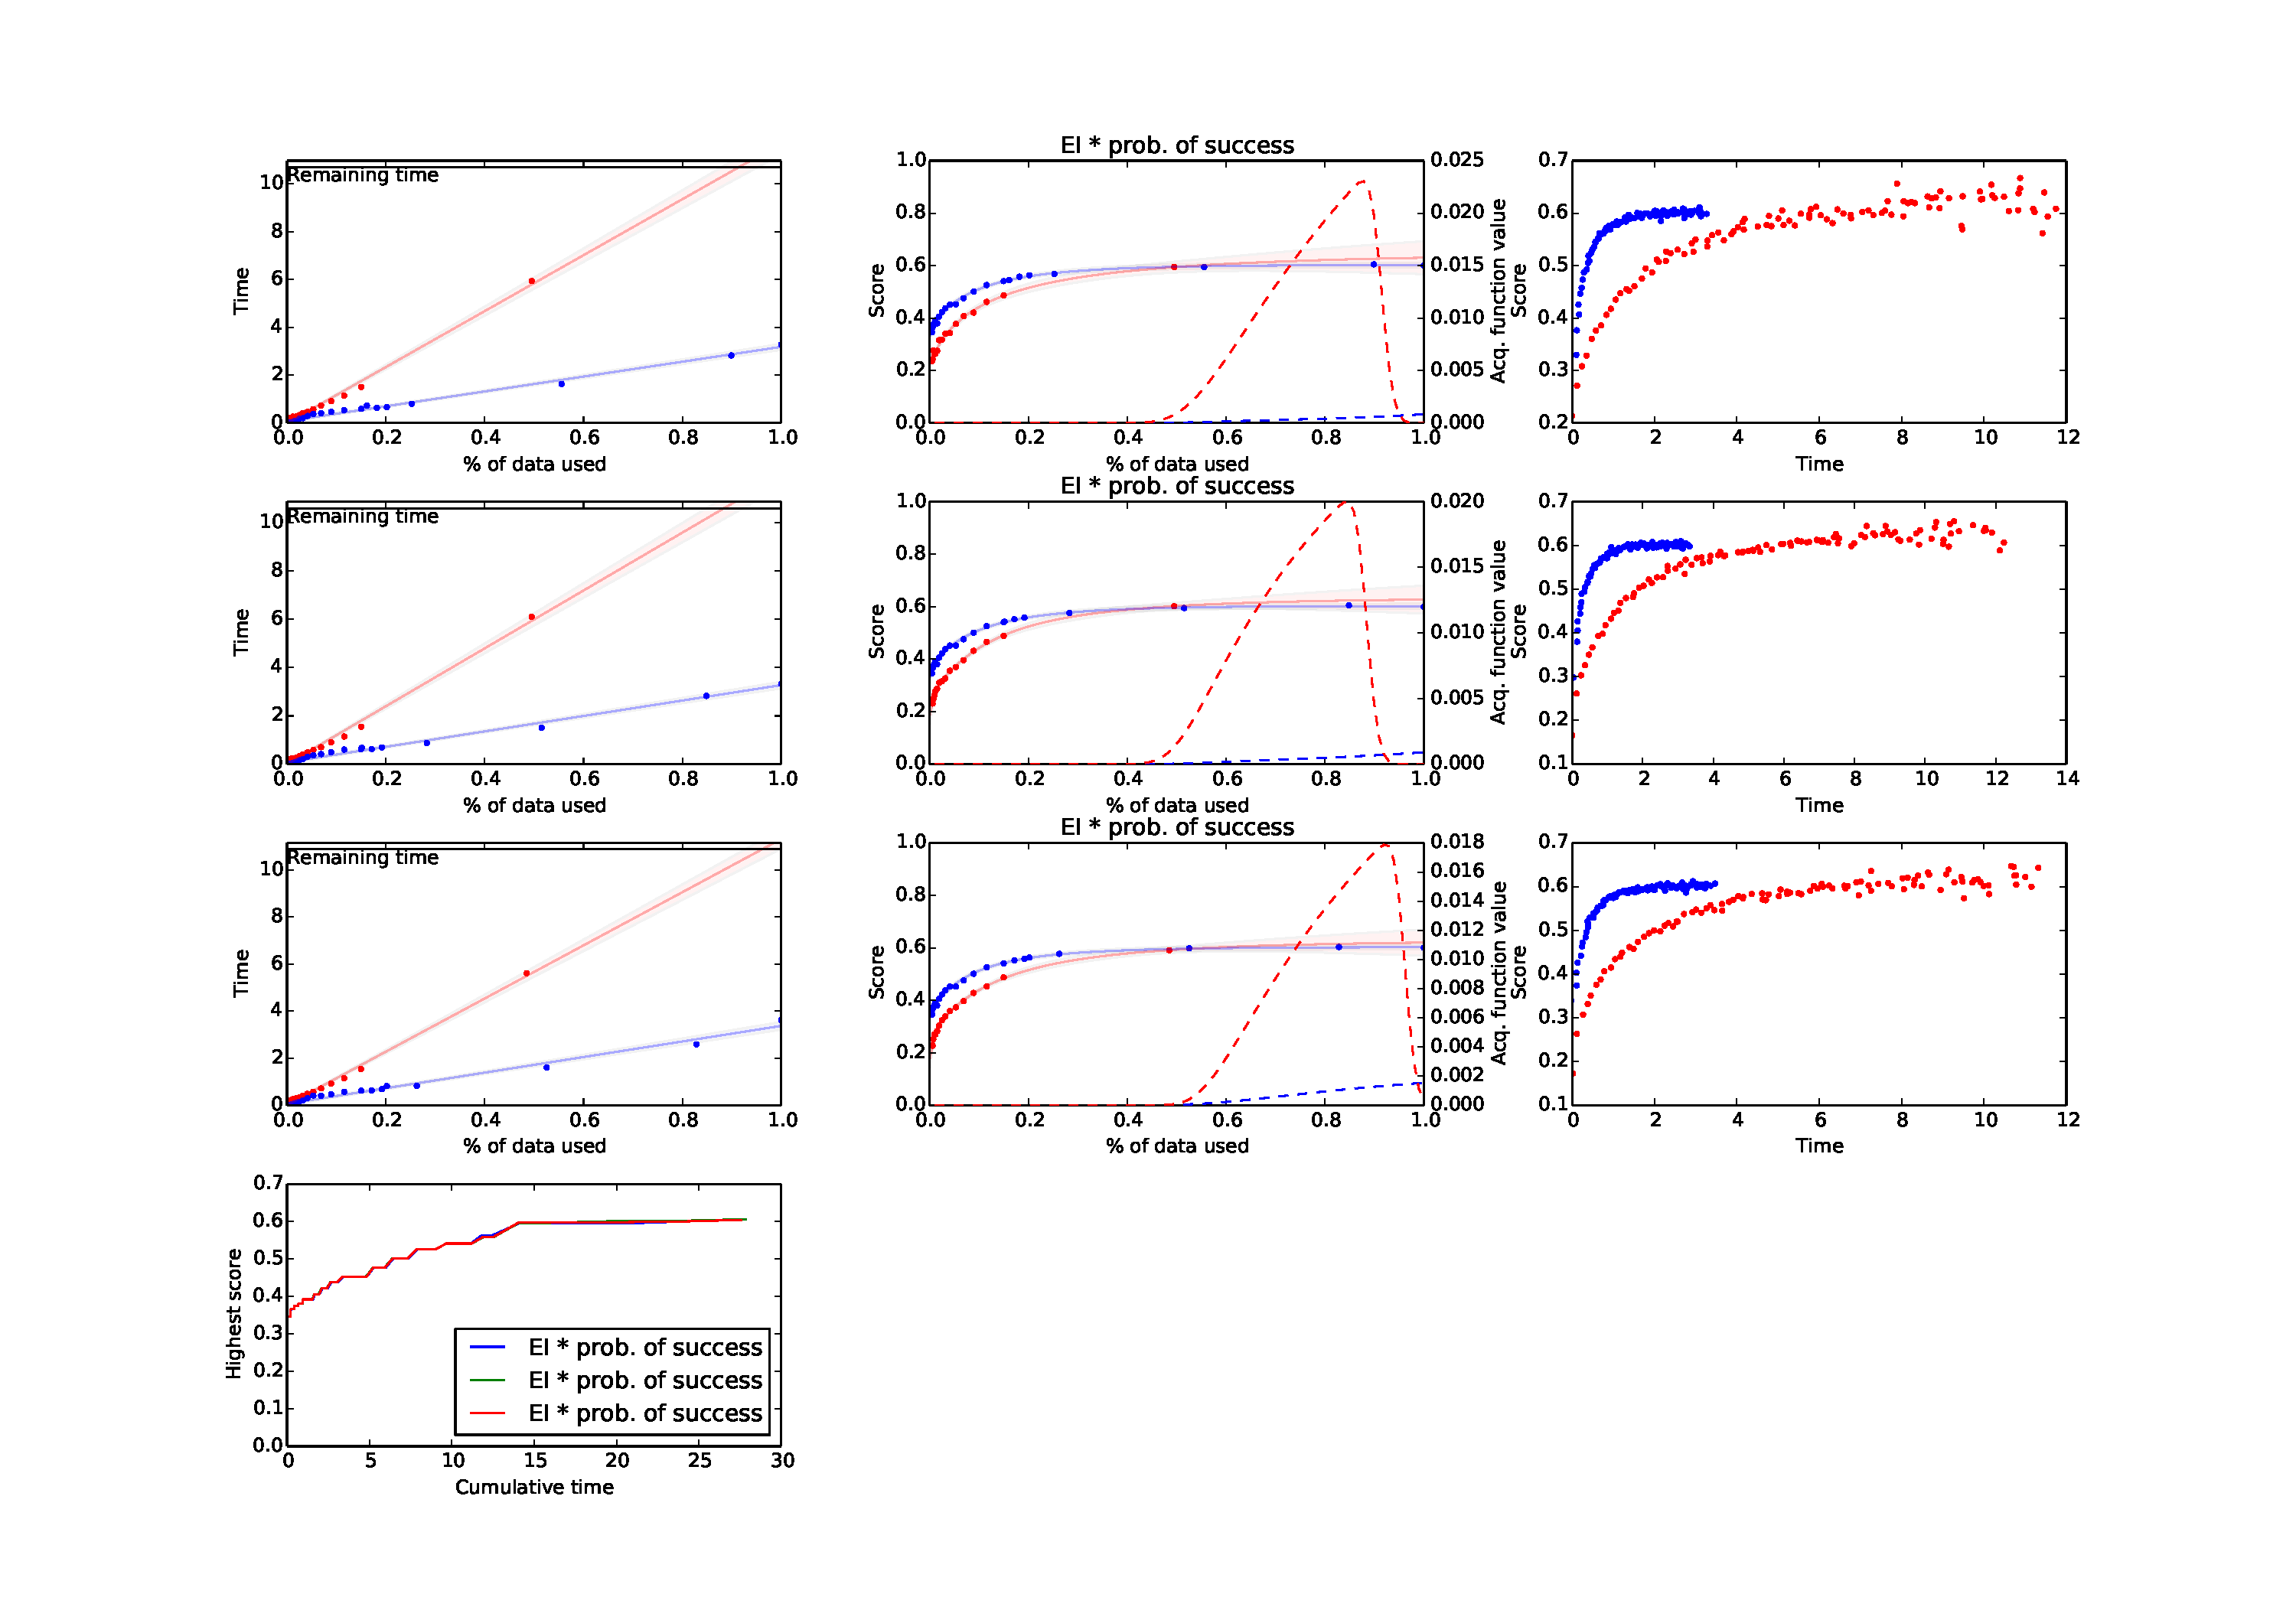
\includegraphics[trim=140 710 493 55,clip,width=\textwidth]{figures/ei_probofsuccess2.pdf}
  \caption{Expected improvement times probability of success}
  \label{sched:expimprpertime02}
\end{figure}

Figure \ref{sched:expimprpertime02} shows the \texttt{ExpectedImprovementTimesProbOfSuccessScheduler} at a later stage of execution. Logistic regression models have been created with several subsets of the data and the scheduler does not expect much improvement by creating another logistic regression model. It has about 12 seconds to spend on random forest. The runtime for this algorithm exceeds this limit for $x$ values close to 1, which is reflected in the sharp drop off in the acquisition function on the right at around an $x$ value of$0.9$.

\subsubsection{\texttt{MinimeseUncertaintyThenExploitScheduler}}

The \texttt{MinimeseUncertaintyThenExploitScheduler} is the second scheduler implemented in this project that operates on a time budget. Recall that it functions in two stages, exploration and exploitation, that are each allocated time during initialisation.

Figure \ref{sched:exp_then_exp1} shows the scheduler shortly after the burn-in period has finished. To illustrate the behaviour of this scheduler, we use a much larger datasets with $50,000$ samples. The scheduler is given 10 seconds to explore and 30 to exploit the knowledge gained during exploration. Due to the size of the dataset, it is not possible to build a model using all the available data in 30 seconds. This makes it necessary for the scheduler to be smart about where to spend the time allocated for exploitation.

% TODO explain why you sample
% Recall that the means of the sampled meta-models are irrelevant during the exploration phase of the \texttt{MinimeseUncertaintyThenExploitScheduler} and decisions are made solely on the amount of variance at a certain point.

In Figure \ref{sched:exp_then_exp1}, random forests has, on average, higher variance in its models than the blue algorithm. It also takes longer to evaluate, however, which causes its acquisition function to have smaller values as the scheduler computes it as $\sigma/\text{time} \cdot \text{probability of success}$. Note how the acquisition functions for both algorithms sharply drop off as the projected time crosses the current time budget of about 9 seconds. This point is reached for random forests at 0.1 and at 0.2 for logistic regression.



\begin{figure}
\centering
  \includegraphics[trim=140 710 493 55,clip,width=\textwidth]{figures/exp_then_exp1.pdf}
  \caption{The \texttt{MinimeseUncertaintyThenExploitScheduler} after burn-in has finished}
  \label{sched:exp_then_exp1}
\end{figure}

Figure \ref{sched:exp_then_exp2} shows the scheduler at the next iteration. A logistic regression model has been trained with about 8\% of the data. The decrease in variance around this point is clearly visible in the blue acquisition function which has a valley around this point. Now, the large variance of the random forests model causes the red acquisition function to dominate, even though it very quickly drops of as the predicted runtime for random forests exceeds the remaining exploration time of about seven seconds.

\begin{figure}
\centering
  \includegraphics[trim=140 710 493 55,clip,width=\textwidth]{figures/exp_then_exp2.pdf}
  \caption{After creating a logistic regression model}
  \label{sched:exp_then_exp2}
\end{figure}


In Figure \ref{sched:exp_then_exp3}, the scheduler has created a random forests model at the point where the red acquisition function shown in Figure \ref{sched:exp_then_exp2} has its maximum. This required all the remaining exploration time and the scheduler has now switched to the exploration phase. This is reflected in the remaining time which has been set to 30 seconds. Using this time, the scheduler tries to create the best model it can using its time budget, calculated as the score mean times the probability of success.

The acquisition functions for both logistic regression and random forests reflect the mean of the means of the sampled score models until the predicted time exceeds 30 seconds and the probability of success quickly goes to zero. The scheduler predicts the best model to be a random forests model created with about 23\% of the available data.

\begin{figure}
\centering
  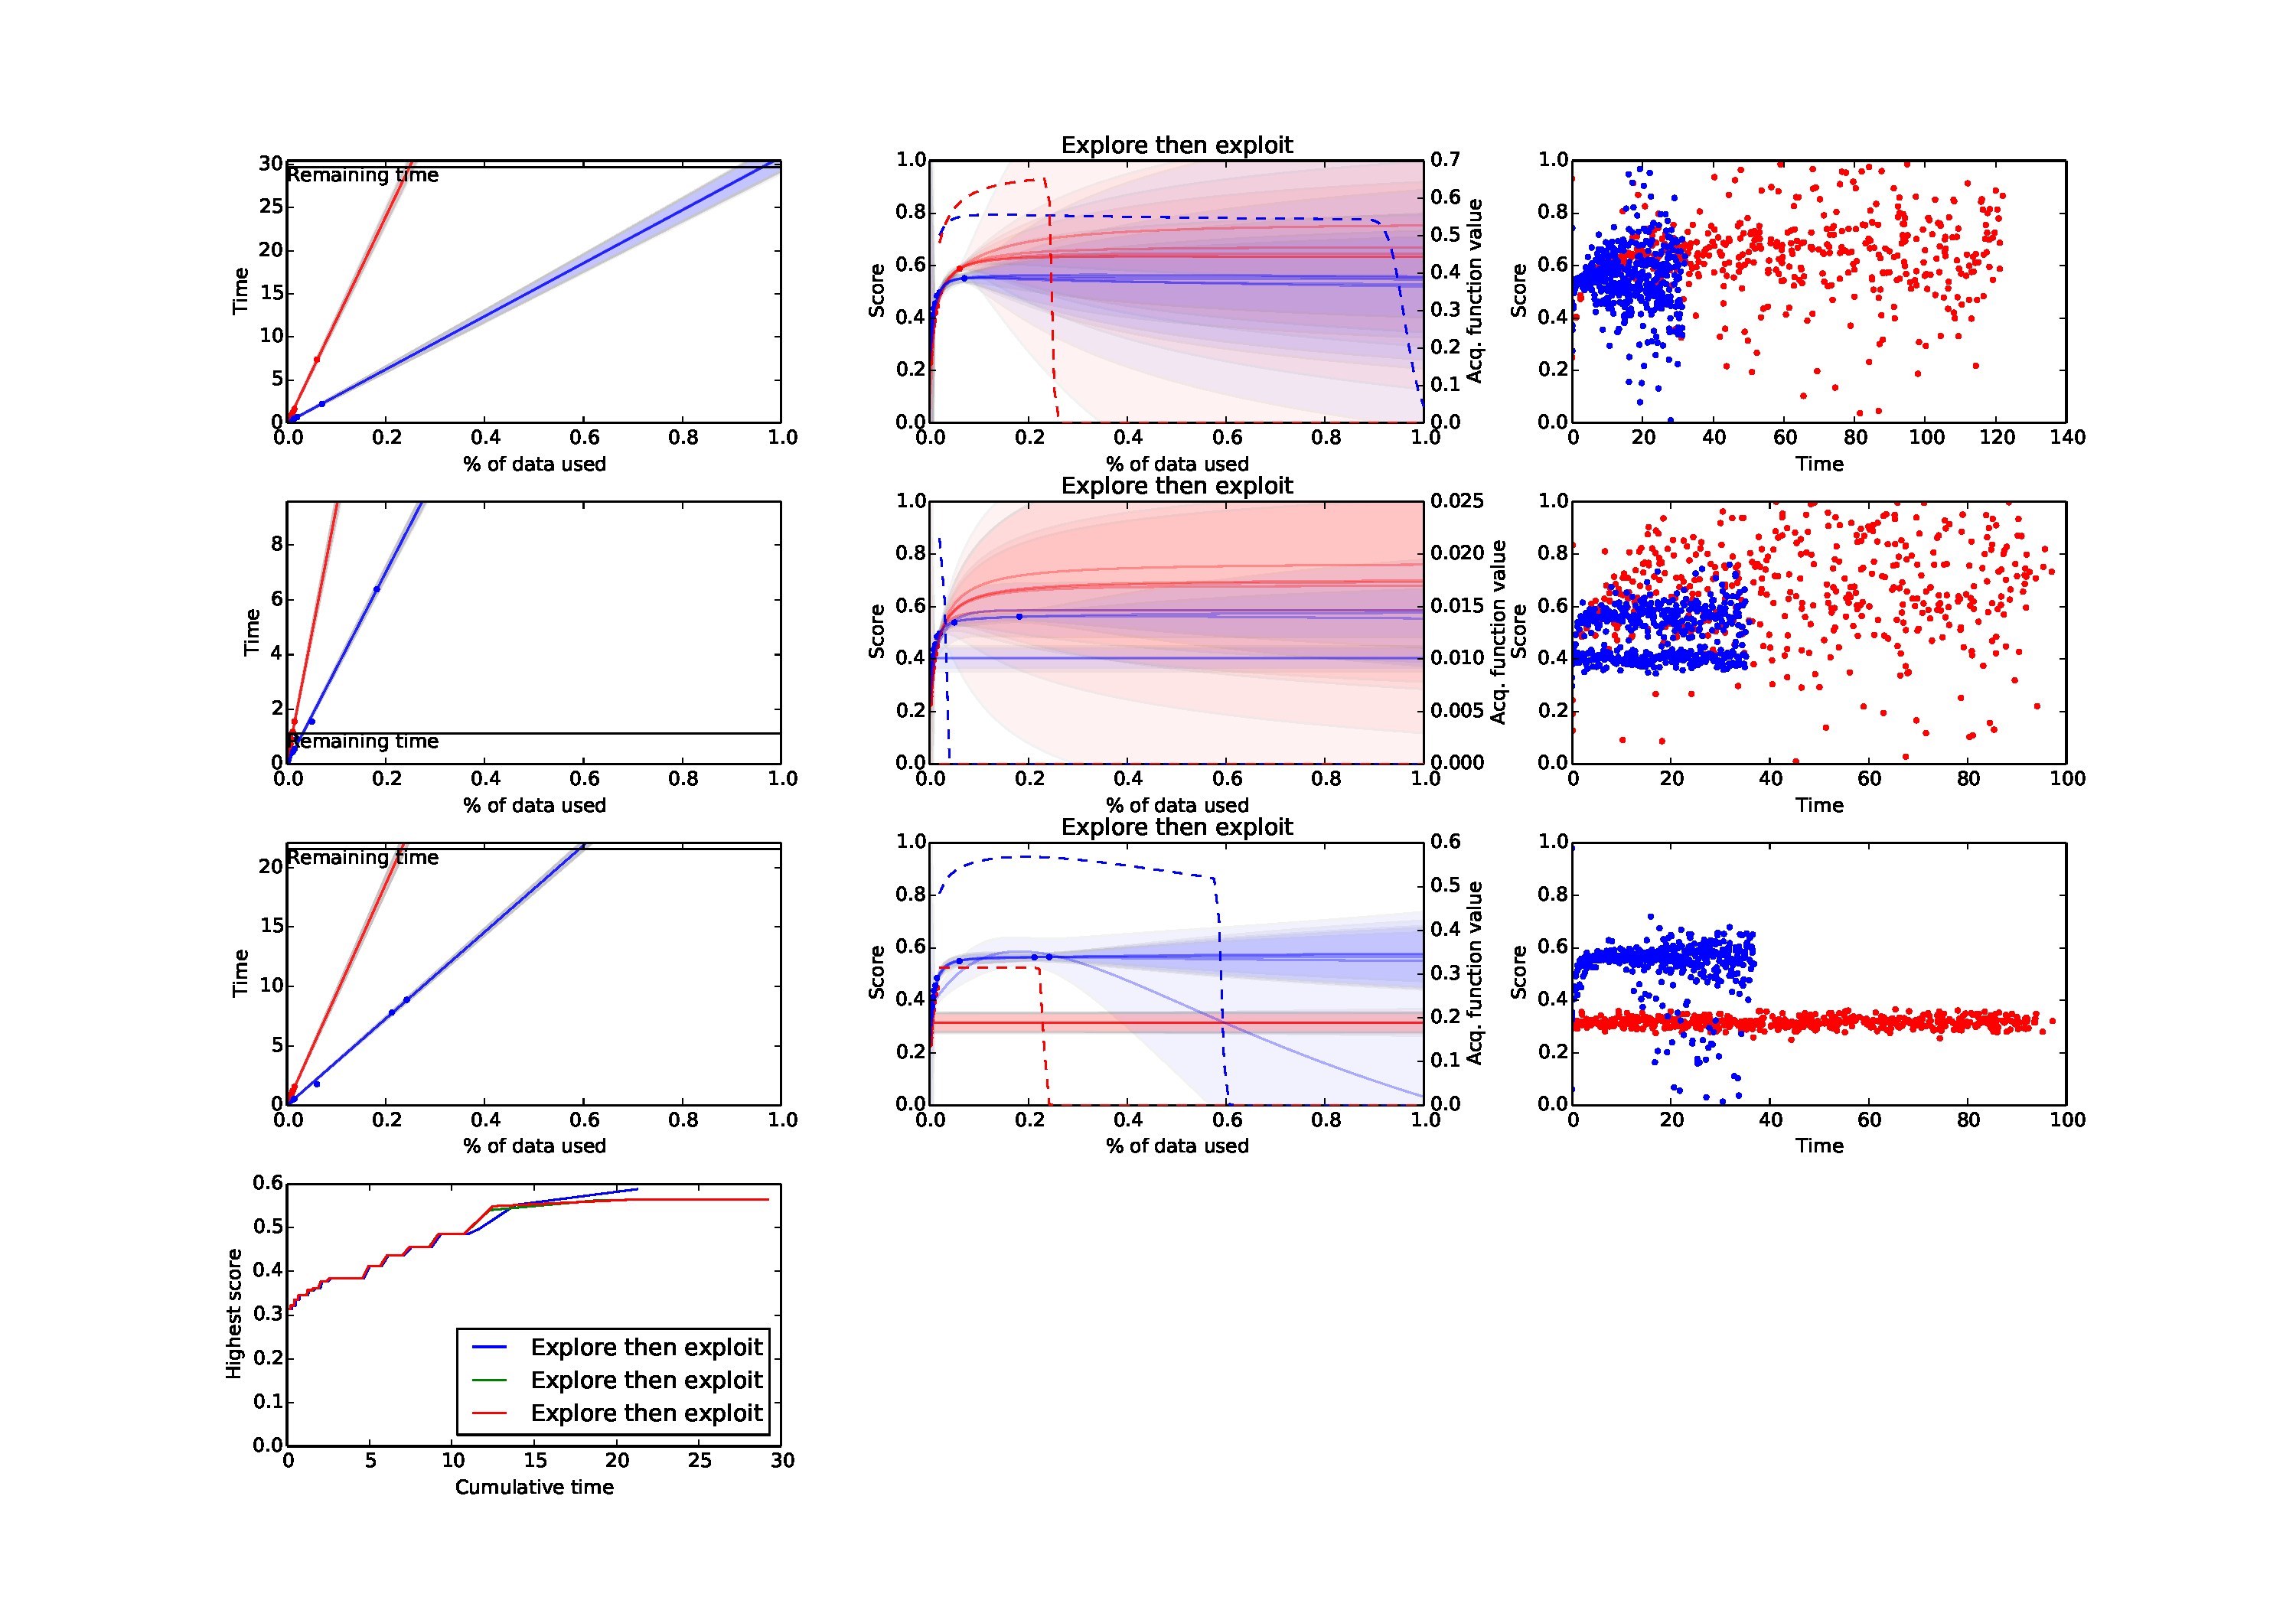
\includegraphics[trim=140 710 493 55,clip,width=\textwidth]{figures/exp_then_exp3.pdf}
  \caption{The exploitation phase}
  \label{sched:exp_then_exp3}
\end{figure}



\subsection{Scheduler Performance}
In this section, we evaluate the heuristics for the two approximation trade-off goals described in the introduction to this report: anytime and contract algorithms.


\subsubsection{Anytime algorithms}

\begin{figure}
\centering
  \includegraphics[trim=0 0 0 0,clip,width=.6\textwidth]{figures/constructed_dataset_anytime.pdf}
  \caption{Score data for one of the datasets used to test the anytime heuristic}
  \label{constructed_dataset_anytime}
\end{figure}

Figure \ref{constructed_dataset_anytime} shows score data for a synthetic dataset with 7500 samples, 120 features and 6 classes. This dataset hat the interesting property that while a random forests model on the full data achieves a higher score than a logistic regression model, if we restrict ourselves to 50\% or less of the samples, logistic regression beats random forests.


\begin{figure}
\centering
  \includegraphics[trim=110 50 895 650,clip,width=.6\textwidth]{figures/anytime2.pdf}
  \caption{The highest score over time for two schedulers}
  \label{anytime2}
\end{figure}



Figure \ref{anytime2} compares our anytime heuristic, the \texttt{ExpectedImprovementTimesProbOfSuccessScheduler}, against a baseline of a \texttt{FixedSequenceScheduler} for this dataset. After the burn in period ends after about 25 seconds, the \texttt{ExpectedImprovementTimesProbOfSuccessScheduler} immediately constructs much better models than the \texttt{FixedSequenceScheduler}. Eventually, both schedulers reach 100\% of data with both random forests and logistic regression, at which point they achieve the same score\footnote{In Figure \ref{anytime2}, the last model the \texttt{FixedSequenceScheduler} scheduler creates is slightly better than that of the \texttt{ExpectedImprovementTimesProbOfSuccessScheduler}. This is due to variance in random forests models.}




\subsubsection{Contract algorithms}

We reuse the dataset shown in Figure \ref{constructed_dataset_anytime} to test our contract heuristic, using only 5000 of the 7500 samples, however, which moves the point at which random forests overtake logistic regression to about 65\% of data.

We first test our contract heuristic in form of the \texttt{MinimeseUncertaintyThenExploitScheduler} with an exploration time budget of 5 seconds and an exploitation time budget of 12 seconds on the dataset shown in Figure \ref{constructed_dataset_anytime}. After finishing exploring, it has reached the state shown in Figure \ref{explexlp0_1}. The acquisition functions shown on the right plot form the basis for the decision it faces next: where to spend its exploitation time. The heuristic predicts that at 80\% of data, a random forests model will be better than the logistic regression model it created in the last iteration.

\begin{figure}
\centering
  \includegraphics[trim=120 510 500 40,clip,width=\textwidth]{figures/explexlp0_1.pdf}
  \caption{The \texttt{MinimeseUncertaintyThenExploitScheduler} after finishing exploring}
  \label{explexlp0_1}
\end{figure}

The final state of the scheduler is shown in Figure \ref{explexlp0}. 


\begin{figure}
\centering
  \includegraphics[trim=120 510 500 40,clip,width=\textwidth]{figures/explexlp0.pdf}
  \caption{The \texttt{MinimeseUncertaintyThenExploitScheduler} after finishing exploiting}
  \label{explexlp0}
\end{figure}


Figure \ref{explexlp1} shows the final state of running a \texttt{MinimeseUncertaintyThenExploitScheduler} on a synthetic dataset with $50,000$ samples, $80$ features and $5$ classes, giving it 30 seconds to explore and 60 seconds to exploit. It chose to spend its exploitation time budget on constructing a random forests model with about 40\% of the available data. It correctly predicted the time it would take to build this model based on the runtime meta-model it constructed during the exploration phase. This can be seen on the left plot with the right dot at $x=0.4$ marking the final model having taken exactly one minute to build.

\begin{figure}
\centering
  \includegraphics[trim=140 495 493 297,clip,width=\textwidth]{figures/explexlp1.pdf}
  \caption{The \texttt{MinimeseUncertaintyThenExploitScheduler} after finishing exploiting}
  \label{explexlp1}
\end{figure}



Although our anytime and contract heuristics have limitations which we describe in the next section, they still perform to a high standard. The results described above would be difficult to reproduce by hand for a human expert.

\subsection{Limitations}
One limitation of our current system is that it models the function from approximation parameters to runtime as linear in all cases. Clearly, not all machine learning algorithm have linear runtime. As described in the Modelling chapter, we've found a linear model to be adequate 

% TODO linear kernel isn't really correct; in future: model selection (n log n or lin or n^3 etc)
The main limitation of our current heuristics is that they are one-step greedy algorithms. This means that at every step, they greedily maximise the gain they can achieve with their next decision. An optimal strategy, however, would think ahead and consider the state of the world given the possible outcomes of the current and all subsequent decisions. These possible future outcomes would then influence the behaviour of the scheduler at the next decision. 

% TODO mention bandits, cite paper;
% TODO JAMES is it correct that the contract heuristic could then automatically balance expl/expl? what about anytime

Considering all these potential states exhaustively is an entirely infeasible problem. We return to this problem when suggesting future work based on the results of this project in the next chapter.



\section{Challenges}
One challenge we faced during the course of this problem resulted from our choice to implement our program in more than one programming language. Python's \texttt{subprocess} library, which we used to call Matlab as described in the Scheduling chapter, is unintuitive to use and often caused zombie children of our main program to accumulate. 

Matlab, on the other side of our interoperability structure, is clearly not very well suited for reading and writing JSON data. Currently, we have to append an empty cell array to a Matlab array that contains only one element when exporting it to prevent it from being exported as an individual object. This is an unsatisfying workaround to which the only true solution is to rewrite the Matlab code in Python.

Implementing the gradients of the hyperparameters to our kernel also proved to be challenging. Even though we are not currently using them, we originally assumed we would use GPML's optimisation function which relies on gradient information. To test our gradient implementation and ensure its correctness, we used a script provided by the creators of GPML that checks kernel gradients\footnote{This script can be downloaded at http://learning.eng.cam.ac.uk/carl/code/minimize/checkgrad.m}. Although they are not currently used in our system, they are available for further development.

Another challenge we encountered during data collection for this project were unexplainable changepoints in the linear growth of the runtime. Figure \ref{time_hinge} shows examples of this effect.

This problem was very hard to investigate. We strongly suspect it to stem from the particularities of the scikit-learn implementations and our computer specifications. It  disappeared when executing the same algorithm/parameter combinations on the EC2 instance and even on our local computer, small changes in hyperparameters often caused the problem to disappear. One possible explanations is an implementation that changes from one routine to another once some kind of threshold is reached. Caching-related effects are another possibility.

As this problem occurred rarely and did not have a noticeable impact on the performance of our system, we did not investigate it further.


\begin{figure}
\centering
\begin{subfigure}{.45\textwidth}
  \centering
  \includegraphics[trim=65 200 30 200,clip,width=\textwidth]{figures/time_dropoff1.pdf}
  \caption{$500$ features, $15,000$ samples}
  \label{time_dropoff1}
\end{subfigure}%
\begin{subfigure}{.45\textwidth}
  \centering
  \includegraphics[trim=65 200 30 200,clip,width=\textwidth]{figures/time_dropoff2.pdf}
  \caption{$500$ features, $10,000$ samples}
  \label{time_dropoff2}
\end{subfigure}
\caption{Non linear behaviour in the growth of the blue line}
\label{time_hinge}
\end{figure}




\chapter{Conclusion and Future Work} 
\section{Conclusions}
In this project, we have succeeded in
\begin{itemize}
	\item creating a covariance function for Gaussian processes that can model the exponential behaviour of learning algorithm accuracy as a function of its appoximation parameters
	\item developing a heuristic that uses this kernel to solve the anytime problem of obtaining good solution fast and quickly improving the models generated during the learning process
	\item developing a heuristic that can generate solutions to the contract style problem of learning within a given time budget
\end{itemize}





\section{Future Work}
One straightforward way our system could be extended is by considering more algorithms besides logistic regression and random forest. Scikit-learn contains implementations of a great number of other machine learning algorithms that could be added to the current list of algorithms with little additional work. One challenge in this is to make the graphical output of the program stay readable while more models and lines are added.

Similarly, the program could be extended to consider additional approximation parameters besides the percentage of data, both individually and in combination with other parameters. The groundwork for this has been laid in this project by fitting exponential mixture kernels to 2D data, but additional investigations on how the approximation parameters influence each other would likely be necessary. This would likely require entirely new ways of visualising the output as it is very difficult to plot functions that take more than one argument.

The heuristics implemented in this project are one step greedy heuristics, meaning they greedily search for maximum gain at every step. This is not the optimal behaviour to find a solution to the problems considered in this report. To find an optimal solution, one instead has to solve the multi-step problem of considering the future states after the possible outcomes at the current step. For each of these future state, one has to consider the states two iterations ahead, recursively considering all future outcomes.

This problem is unlikely to have an analytic solution and is therefore intractable to compute. A solution to this is to develop multi-step heuristics using meta meta machine learning, i.e. using machine learning to learn heuristics that choose which learning algorithms to run in what order. This could be achieved using reinforcement learning techniques by making the information at every step available to the reinforcement learning algorithm and judging its decisions by evaluating its decisions once training has finished.

% TODO possible goal: fixed error, trade off data and time


\appendix
\singlespacing

% TODO ADD more references

\bibliographystyle{unsrt} 
\bibliography{references}


\end{document}
